% !Mode:: "TeX:UTF-8"
%!TEX program  = xelatex
% 编译：xelatex -> bibtex -> xelatex -> xelatex
\documentclass[bwprint]{gmcmthesis}

\usepackage{tikz}
\usetikzlibrary{arrows.meta,positioning,calc,fit,backgrounds}
\usepackage{algorithm}
\usepackage{algpseudocode}
\usepackage{csvsimple}
\usepackage{float}
\usepackage{longtable}
\normalem % ulem 默认会把 \emph 变成下划线，这里恢复成正常强调
\AtBeginEnvironment{table}{\small\setlength{\tabcolsep}{4pt}} % 表格用五号左右字号
\setcounter{tocdepth}{2}
\setlength{\emergencystretch}{2em}

% 待填项：用醒目的红字标出，提交前务必全部替换
\newcommand\todo[1]{\textcolor{red}{\textbf{【待填：#1】}}}

\renewcommand{\algorithmicrequire}{\textbf{输入：}}
\renewcommand{\algorithmicensure}{\textbf{输出：}}
\floatname{algorithm}{算法}

\title{面向局部模态缺失的多模态情感预测与证据追溯}
\baominghao{26XXXXXXXXX} % 参赛队号
\schoolname{XX大学}      % 学校名称
\membera{XXX}            % 队员A
\memberb{XXX}            % 队员B
\memberc{XXX}            % 队员C

% ------------------------------------------------------------------
% 封面：沿用原稿当届官方封面上的四个标识（figures/cover_logos.pdf，矢量裁取）；
% 标题文字改为第二十三届。拿到当届官方 Word/PDF 封面时以官方为准。
% ------------------------------------------------------------------
\makeatletter
% 模板的 \thesection 自带尾点，交叉引用会变成“第5.章”，这里把点挪到标题格式里
\renewcommand\thesection{\arabic{section}}
\newcommand\secdot{.}
\def\@seccntformat#1{\csname the#1\endcsname\csname secdot@#1\endcsname\ \ }
\def\secdot@section{\secdot}
\newcommand\tocsecdot{.}
\titlecontents{section}[0pt]{\vspace{2mm}\bfseries\heiti}
  {\thecontentslabel\tocsecdot\hskip.5em}{}{\titlerule*[0.5pc]{.}\contentspage}
\renewcommand\gmcm@ges@string@contents{%
  {\zihao{-2}中国研究生创新实践系列大赛}\\[6pt]
  “华为杯”第二十三届中国研究生\\[2pt]
  数学建模竞赛}
\def\ge@maketitle{%
  \newpage
  \if@gmcm@preface
  \setcounter{page}{0}%
  \def\thepage{0}%
  \thispagestyle{empty}%
  \begin{center}
    {
\includegraphics[width=0.78\textwidth]{figures/cover_logos}}
    \vskip2.2cm
    {\xinwei\zihao{2} \gmcm@ges@string@contents \par}
  \end{center}
  \vskip2em
  \renewcommand\arraystretch{1.3}%
  \noindent\begin{tabularx}{\textwidth}{lX}
    \zihao{-2}\bfseries 学\qquad 校&\zihao{-2}\bfseries\gmcm@tokens@schoolname\\
    \hline\\[-15pt]
    \zihao{-2}\bfseries 参赛队号&\zihao{-2}\bfseries\gmcm@tokens@baominghao\\
    \hline\\[-15pt]
    \multirow{3}{*}{\zihao{-2}\bfseries 队员姓名}&\zihao{-2}\bfseries 1. \gmcm@tokens@membera\hfill\null\\
    \cline{2-2}\\[-15pt]
    &\zihao{-2}\bfseries 2. \gmcm@tokens@memberb\hfill\null\\
    \cline{2-2}\\[-15pt]
    &\zihao{-2}\bfseries 3. \gmcm@tokens@memberc\hfill\null\\
    \hline
  \end{tabularx}
  \fi
  \makenametitle}
\def\makenametitle{%
  \newpage
  \setcounter{page}{1}%
  \vspace*{-1.2cm}
  \begin{center}
    {\xinwei\zihao{3} \gmcm@ges@string@contents \par}
  \end{center}
  \vskip0.2cm
  \begin{center}\begin{tabularx}{.95\textwidth}{@{}lX@{}}
    {\zihao{4} 题\qquad 目} &\hfill\zihao{3}\heiti \@title\hfill\null\\
    \cline{2-2}
  \end{tabularx}\end{center}
  \vskip-0.4cm}
\makeatother

\begin{document}

\maketitle

\begin{abstract}
真实视频里，文本、声音和画面并不总能同时观测，情感判断还需要能回到原始素材上核对。本文把三问当成一条链：构造可反查的特征，在局部缺失下预测情感，再给出可回溯的解释。

针对问题一，我们用 WhisperX 对给定转写做强制对齐得到词级时间，把 BERT 子词、openSMILE 声学帧和 OpenFace 人脸动作单元帧按词时间窗对齐池化，得到768、25、35维特征，每个位置都能反查到原词、秒数和帧号。100条全部保留：77条正常、19条需复核、4条找不到达标的人脸帧；文本100条可用，声学、视觉各92条可用。人工核验的583个词全部通过。

针对问题二，我们把补齐填充、原生不可观测、人为遮蔽三种零值分开记录，建立掩码感知的池化双头模型 PM-B2，同时输出类别和强度。在7种遮蔽组合、3种比例、3种位置构成的63档缺失面板上，三种子平均 macro-F1 为0.5752$\pm$0.0013、MAE 为0.6213$\pm$0.0123，均优于7个基线；测试集完整输入 macro-F1 为0.6147、MAE 为0.6485。遮蔽含文本时 F1 比只遮蔽声学或视觉低约0.04，缺失比例从10\%增至50\%时 F1 由0.5905降到0.5595，位置的影响在验证集上不到0.005。主要错误在中性类，测试集中性召回仅0.361。另做的15种改进配置中，完整输入 F1 最高达0.6244，但在更严格的整模态压力面板上只有0.4139，故未替换正式模型。附件3的30条预测为正向14、中性10、负向6条。

针对问题三，我们固定完整输入下的预测类别，对三模态的8个子集精确计算 Shapley 值，全部样本的效率恒等式误差不超过$10^{-6}$；验证集上文本对分类的平均贡献约为声学、视觉的6～7倍。在附件4上删除得分最高的30\%位置，目标类概率平均下降约0.14，删除随机位置仅约0.03。附件4中以非文本为主导的5条样本置信度都不超过0.565，其余15条平均为0.79。文字与声音不符的样本15，其词时间被人工核验全部拒绝，只给出位置级证据。

\keywords{多模态情感分析；强制对齐；局部模态缺失；池化双头模型；Shapley 归因；删除检验}
\end{abstract}


\pagestyle{plain}
\tableofcontents
\newpage

% ==================================================================
\section{问题重述}
% ==================================================================

\subsection{问题背景}

人表达情绪时，说了什么、用什么语气说、说话时脸上是什么表情，三者往往同时起作用。多模态情感分析就是把这三路信号放在一起判断，它是人机对话、具身智能等应用的基础环节。CMU-MOSEI 是这一方向最常用的英文视频数据集之一\cite{zadeh2018mosei}。

可是到了真实视频上，事情并不整齐。三路信号的时间尺度不同：文本以词为单位，声音以毫秒为单位分帧，画面以固定帧率抽取；片段里还常有静音、人脸出画、转写与声音对不上的情况。这带来两个直接的问题：模型在某一路局部缺失时是否还靠得住，以及模型给出判断后，能不能指出它依据的是哪句话、哪段声音、哪几帧画面。

赛题围绕这两个问题设置了三项任务：从原始视频提取特征并做时序对齐，在模态局部缺失下做鲁棒预测，以及做可解释的预测。本文依次完成这三项任务。

\subsection{数据说明与使用边界}\label{sec:data}

赛题提供四个附件，本文对它们的用法见表\ref{tab:data}。附件2的对齐版特征 aligned\_50.pkl 共4850条，训练集、验证集、测试集分别为3395、728、727条。

\begin{table}[htbp]
\centering
\caption{题目附件及本文的使用方式}
\label{tab:data}
\begin{tabularx}{\textwidth}{l>{\raggedright\arraybackslash}p{3.3cm}c>{\raggedright\arraybackslash}X}
\toprule
数据 & 规模与结构 & 标签 & 本文用途 \\
\midrule
附件1 & 100段原始视频，37个源视频 & 有 & 只用于问题一的原始特征、时间映射与异常分析，不进入问题二的训练 \\
附件2 & 训练3395、验证728、测试727；50个位置 & 有 & 训练集拟合参数，验证集选结构和检查点；测试集只在模型冻结后评估一次 \\
附件3 & 30条对齐特征 & 无 & 问题二的缺失专项推理 \\
附件4 & 20条对齐特征及原始视频 & 无 & 问题三的预测、解释与人工时间核验 \\
\bottomrule
\end{tabularx}
\end{table}

有两点需要事先说明。第一，测试集在模型冻结后我们评估过一次，已经看过结果，所以后面的改进实验一律不再使用它，也不把它当作从未接触过的盲测集。第二，问题一自己提取的声学特征是25维，附件2的声学特征是74维，两者都来自声音，却不是同一套特征；视觉虽然都是35维，含义也不一定相同。问题二、三只用附件2的现成特征，不与问题一的特征混用。

\subsection{需要解决的问题}

\textbf{问题一：}基于附件1的原始视频，建立文本、语音、视觉三模态情感特征提取与时序对齐的数学模型，说明原始样本的处理流程、各模态特征的定义与提取方法、跨模态对齐的规则与实现；生成的特征要做到样本覆盖完整、时序组织可核验、方法可复现，并用典型样本展示对齐效果。

\textbf{问题二：}针对文本、语音或视觉中部分连续时间段不可用的情形，构建鲁棒的情感预测模型，同时输出极性和强度；分析缺失模态类型、缺失位置、缺失时长对性能的影响；对附件3完成推理。

\textbf{问题三：}针对三模态完整但决策依据难以追溯的情形，构建可解释的情感预测模型，在输出极性与强度的同时，定量给出各模态的作用程度、主要参考模态，以及能对应到原始文本片段、语音时段或视觉关键帧的关键证据；对附件4完成推理。

% ==================================================================
\section{问题分析}
% ==================================================================

\subsection{问题一的分析}

问题一的难点在于让每个特征位置都能回到原始素材上。具体有三层。

第一层是时间从哪里来。文本本身没有时间戳。最省事的办法是把整段视频均匀切成若干份，按顺序分给各个词，但这样会给停顿、静音、人不在画面里的时段凭空编出“词时间”。我们更希望每个词的时间都有依据。

第二层是一词多位。BERT 按子词切分，一个英文词可能占两三个位置，这些位置应当共享同一个词的时间窗，而不是各自再切一段。

第三层是提取失败。有的片段没有语音，有的转写和声音对不上，有的全程找不到清晰的人脸。这些情况如果都用零填充，下游就分不清“这里没有表情”和“这里根本没提取到”。

据此，问题一的路线是：先用强制对齐工具 WhisperX\cite{bain2023whisperx} 在给定转写上求词级时间，再用字符重叠把子词对到原词，然后把声学帧和人脸动作帧按词时间窗池化到50个位置；凡是拿不到时间或拿不到帧的位置，都显式记录其状态，而不是悄悄补零。

\subsection{问题二的分析}

与问题一不同，问题二直接用附件2现成的50位置特征，重点从“特征怎么来”转到“缺了一段还能不能判断准”。难点有两层。

第一层是零值有三种来源：序列本身较短留下的补齐填充、原始数据里就没有观测、我们为做实验人为遮掉的部分。三者如果混在一起，模型和评估都会被误导。因此我们对每个位置分别记录这三种掩码。

第二层是评估的独立性。同一条样本会在很多个缺失档位里重复出现，同一个源视频也会切出多个片段，它们都不是彼此独立的样本。所以我们对63个缺失档先分别算指标再等权平均，比较两个模型时按源视频成组做配对重抽样。

在模型选择上，张量融合 TFN\cite{zadeh2017tfn}、低秩融合 LMF\cite{liu2018lmf} 和跨模态 Transformer MulT\cite{tsai2019mult} 代表了表达能力逐步增强的几类融合方式。但本题训练样本只有3395条，输入又已经按50个位置对齐，复杂模型不一定占优。我们因此以参数很少的池化双头模型为主线，把低秩融合、文本 BiLSTM、跨模态时序网络等作为同一评估口径下的对照，让数据来决定用哪个。

\subsection{问题三的分析}

与问题二相比，问题三的输入是完整的，难点从“预测得稳”转到“说得清”。这里要回答三个问题：模态重要性的排序针对的是哪一个输出；被选出来的词或帧，删掉以后是不是真的会改变这个输出；给出的时间位置在原始视频里是否真有其事。

这三个问题需要三种不同的检验。模态层面，我们用 Shapley 值\cite{lundberg2017shap}把完整预测与各模态子集预测之间的差分摊给三个模态，三模态只有8个子集，可以精确计算，不需要采样近似。局部证据层面，参照 ERASER\cite{deyoung2020eraser}的做法，用删除高分位置后预测的变化来检验证据是否忠实于模型。时间层面，则由人工对照视频逐词核对。前两项检验的是“模型是不是这么用的”，第三项检验的是“素材里是不是真有这个”，谁也替代不了谁。

\subsection{求解思路}

三问的整体流程如图\ref{fig:flow}所示。

\begin{figure}[htbp]
\centering
\begin{tikzpicture}[
  node distance=3mm,
  box/.style={draw=black!65, rounded corners=2pt, align=flush center, font=\small, inner sep=3pt, minimum height=7.5mm},
  wide/.style={box, text width=13.2cm, fill=black!4},
  q1/.style={box, text width=13.2cm, fill=green!6},
  q2/.style={box, text width=6.2cm, fill=blue!5},
  q3/.style={box, text width=6.2cm, fill=orange!7},
  head/.style={font=\small\bfseries, text width=6.2cm, align=flush center},
  arr/.style={-{Stealth[length=1.8mm]}, draw=black!70, semithick}]
\node[head, text width=13.2cm] (h1) {问题一：原始视频的三模态特征与时间对齐（附件1）};
\node[q1, below=2mm of h1] (p1) {WhisperX 强制对齐给定转写 $\to$ 词级时间；字符重叠 $\to$ 子词对原词};
\node[q1, below=of p1] (p2) {BERT（768维）、eGeMAPS 声学（25维）、OpenFace 动作单元（35维）按词时间窗池化到50个位置};
\node[q1, below=of p2] (p3) {可观测掩码与失败状态、人工核验、100条台账};
\node[wide, below=8mm of p3] (d) {附件2：分离补齐填充、原生不可观测、人为遮蔽三种掩码；训练集拟合、验证集选型};
\node[head, below=5mm of d.south west, anchor=north west] (h2) {问题二：局部缺失下的预测};
\node[head, below=5mm of d.south east, anchor=north east] (h3) {问题三：模态归因与局部证据};
\node[q2, below=2mm of h2] (a1) {PM-B2 池化双头模型与7个基线};
\node[q2, below=of a1] (a2) {63档局部缺失面板、视频级配对重抽样};
\node[q2, below=of a2] (a3) {缺失类型、比例、位置的影响规律};
\node[q2, below=of a3] (a4) {A–E 改进尝试与整模态压力面板};
\node[q2, below=of a4] (a5) {测试集误差分析、附件3推理};
\node[q3, below=2mm of h3] (c1) {固定目标类别，八子集精确 Shapley};
\node[q3, below=of c1] (c2) {逐位置删除：高分 / 低分 / 随机对照};
\node[q3, below=of c2] (c3) {子词位置回指原词与音视频帧};
\node[q3, below=of c3] (c4) {人工时间核验（拒绝不可信时间）};
\node[q3, below=of c4] (c5) {附件4预测与解释卡};
\draw[arr] (p1) -- (p2); \draw[arr] (p2) -- (p3);
\draw[arr, dashed] (p3) -- node[right, font=\scriptsize]{特征口径不同，只共享处理思路} (d);
\draw[arr] (d.south -| h2.north) -- (h2.north);
\draw[arr] (d.south -| h3.north) -- (h3.north);
\foreach \x/\y in {a1/a2,a2/a3,a3/a4,a4/a5,c1/c2,c2/c3,c3/c4,c4/c5} \draw[arr] (\x) -- (\y);
\draw[arr, dashed] (a1.east) -- (c1.west);
\end{tikzpicture}
\caption{全文求解思路（中间的虚线箭头表示问题三直接使用问题二冻结的正式模型）}
\label{fig:flow}
\end{figure}

% ==================================================================
\section{模型假设}
% ==================================================================

\begin{enumerate}[label=(\arabic*)]
\item 情感标签对应整个片段，片段内的50个位置共享同一个标签；位置级证据说明模型依赖哪里，不代表该词有单独的情感真值。
\item 同一源视频切出的多个片段之间可能相关，比较模型差异时按源视频成组抽样。
\item 人为遮蔽只改变观察到的特征，不改变标签；全部模态都不可用时，模型返回训练集的类别先验和强度中位数。
\item 转写与声音不符、静音或无人脸时，保留样本及其可用模态，但不为它编造词时间或视频帧。
\item 附件3、4的标签未知，其结果只能检查格式、内部一致性和人工可核对性，不能计算监督意义上的准确率。
\end{enumerate}

\textbf{说明。}假设(2)直接影响区间估计：附件2验证集的728条来自239个源视频，同一视频的片段在说话人、场景上高度相似。如果按条独立重抽样，会把这种相关性当成独立信息，得到过窄的置信区间，所以我们按视频成组抽样。

假设(3)界定了缺失面板回答的是什么问题：在预先设定的遮蔽方式下模型还剩多少能力。真实世界的缺失未必是这样发生的，因此63档结果代表的是这类可控干预下的鲁棒性，不能直接推广到任意缺失机制。

假设(4)在问题一和问题三中都用到了。宁可让一个位置“没有时间”，也不给它一个看起来合理却无法核对的时间，因为后者一旦被当作证据引用，比缺失更难发现。

% ==================================================================
\section{符号说明}
% ==================================================================

\begin{table}[htbp]
\centering
\caption{主要符号说明}
\label{tab:symbols}
\begin{tabularx}{\textwidth}{c>{\raggedright\arraybackslash}X}
\toprule
符号 & 含义 \\
\midrule
$i$，$t$（或 $p$），$m$ & 样本序号、50个位置的序号、模态 $m\in\{T,A,V\}$（文本、声学、视觉） \\
$D_i$ & 问题一：第 $i$ 段视频的时长 \\
$[s_{ij},e_{ij})$ & 问题一：第 $j$ 个原词的起止时间 \\
$\mathcal{I}_{ip}^m$，$L_i^m$ & 问题一：位置 $p$ 的池化帧集合；模态 $m$ 的有效位置数 \\
$\ell_{imt}$，$o_{imt}$，$s_{imt}$ & 布局掩码、原生可观测掩码、人为遮蔽掩码 \\
$a_{imt}$ & 实际送入模型的可用掩码，$a=o(1-s)$ \\
$\boldsymbol{\mu}_{im}$，$\boldsymbol{d}_{im}$ & 模态 $m$ 可观测位置的均值池化与“均值+标准差”池化向量 \\
$\boldsymbol{p}_i$，$\hat c_i$，$\hat y_i$ & 三类概率、预测类别、预测强度 \\
$y_i$，$c_i$ & 真实强度（$[-3,3]$）与真实类别 \\
$r$，$\rho_{im}$ & 名义缺失比例；实际删除比例 \\
$\mathcal{K}_{PM}$ & 局部遮蔽面板：在被选模态内删除连续窗口，共63档 \\
$\mathcal{K}_{LH}$ & 整模态保留压力面板：只保留子集 $S$，其余模态整路关闭，共63档 \\
$v_i^h(S)$，$\phi_{i,m}^h$ & 只保留模态子集 $S$ 时的输出；模态 $m$ 的 Shapley 贡献，$h\in\{\mathrm{cls},\mathrm{reg}\}$ \\
$c_i^\star$，$R_k$ & 完整输入下的预测类别；局部得分最高的前 $k$ 个位置 \\
\bottomrule
\end{tabularx}
\end{table}

注：此为本文的主要符号，其他符号在正文首次出现处说明。

% ==================================================================
\section{问题一：原始视频的三模态特征与时间对齐}\label{sec:q1}
% ==================================================================

问题一要从100段原始视频得到固定长度的三模态特征，并让每个位置都能回到原始的词、声学帧和视频帧。本章先给出词级时间的求法，再给出三路特征的构造和池化规则，最后用一条典型样本和全量台账检验结果。需要强调的是，本章的目标是构造可以逐条核对的原始数据映射，而不是去模仿附件2特征的数值；问题二的模型也不在这些特征上训练。

\subsection{原始样本与处理流程}

附件1的100段视频来自37个源视频，以二元组 $i=(\text{video\_id},\text{clip\_id})$ 唯一标识。转写文本和情感标签一律取自题目给定的 label-100.xlsx，不用自动语音识别的结果替换原文。每段视频先用 ffprobe 读取时长 $D_i$，再用 ffmpeg 抽出16 kHz 单声道音频。按 ffprobe 的读数，100段时长在2.257～29.288秒之间，合计约787秒；这一范围与赛题说明中给出的2.648～34.567秒不完全一致，本文以实际文件的读数为准。

整条处理链分三步：先求词级时间（第\ref{sec:q1time}节），再把声学帧和视觉帧按词时间窗池化到子词位置（第\ref{sec:q1feat}节），最后为每个位置记录能否观测以及失败原因（第\ref{sec:q1mask}节）。三步完成后，每个有效位置都挂着一条“原文字符 $\to$ 词 $\to$ 子词位置 $\to$ 音视频帧”的反查链。

\subsection{词级时间映射}\label{sec:q1time}

以视频起点为零时刻，把原转写按非空白字符切成词 $w_{ij}$，同时保存每个词在原文中的字符区间 $[c_{ij},d_{ij})$。WhisperX\cite{bain2023whisperx} 对给定转写做强制对齐，求出每个词的起止时间。首轮没有全部对齐成功时，程序会利用静音边界把句子切开后重新对齐；静音边界只用来辅助切句，不作为最终的词时间，我们也不用均匀切分去补造时间。规范化词串匹配以后，只对拿到有效数值区间的词记录 $[s_{ij},e_{ij})$。

文本用冻结的 bert-base-uncased 取最后一层隐状态\cite{devlin2019bert}。WordPiece 编码加上 \texttt{[CLS]} 和 \texttt{[SEP]} 后长度固定为50，最多保留48个正文子词，不足的位置补齐。设位置 $p$ 的子词在原文中的字符区间为 $[u_{ip},v_{ip})$，按字符重叠最大的原则确定它属于哪个原词：
\begin{equation}\label{eq:overlap}
j_i(p)=\mathop{\arg\max}_{j:\ [u_{ip},v_{ip})\cap[c_{ij},d_{ij})\neq\varnothing}\ \big|[u_{ip},v_{ip})\cap[c_{ij},d_{ij})\big|.
\end{equation}
如果某个位置和任何原词都没有重叠，或者对应的词没有有效时间，就保留这个位置和原因，但不给它写入音视频时间。\texttt{[CLS]}、\texttt{[SEP]} 和补齐位也不冒充任何词。文本矩阵 $X_i^T\in\mathbb{R}^{50\times768}$ 的补齐行置零，同时保存词元编号、注意力掩码和分段编号。

\subsection{声学与视觉特征及词窗池化}\label{sec:q1feat}

声学特征用 openSMILE\cite{eyben2010opensmile} 的 eGeMAPSv02 低层描述量，共25维\cite{eyben2016gemaps}，包括音高、响度、共振峰、频谱斜率等与情感表达关系密切的量。视觉特征用 OpenFace 2.0\cite{baltrusaitis2018openface} 的人脸动作单元（AU），其中17维是强度、18维是出现标志，共35维；动作单元直接对应皱眉、嘴角上扬这类面部动作，比笼统的人脸框统计量更贴近表情。

声学帧的时刻取其时间窗的中点 $\tau_{ik}^A$，视频帧的时刻取 OpenFace 给出的时间戳 $\tau_{ik}^V$。视觉帧必须同时满足三个条件才算有效：提取成功、置信度不低于0.8、数值有限。设 $\boldsymbol z_{ik}^m$ 为模态 $m\in\{A,V\}$ 的第 $k$ 帧向量，$b_{ik}^m$ 为其有效标志，则位置 $p$ 的池化帧集合与特征为
\begin{equation}\label{eq:pool}
\mathcal{I}_{ip}^m=\big\{k:\ s_{i,j_i(p)}\le\tau_{ik}^m<e_{i,j_i(p)},\ b_{ik}^m=1\big\},\qquad
\boldsymbol x_{ip}^m=\begin{cases}\dfrac{1}{|\mathcal{I}_{ip}^m|}\displaystyle\sum_{k\in\mathcal{I}_{ip}^m}\boldsymbol z_{ik}^m, & |\mathcal{I}_{ip}^m|>0,\\[10pt]\mathbf{0}, & |\mathcal{I}_{ip}^m|=0.\end{cases}
\end{equation}

同一个词切出的几个子词继承同一个词时间窗，因此会引用同一批声学帧和视频帧。这是有意为之：它们本来就是同一个词，时间上不该被人为拆开；但也要注意，这几个位置并不是几次独立的观测。最终得到 $X_i^A\in\mathbb{R}^{50\times25}$、$X_i^V\in\mathbb{R}^{50\times35}$，并为每个有效位置保存声学帧数、视频起止帧号和原始秒数。

\subsection{可观测状态与有效长度}\label{sec:q1mask}

零值本身说明不了“这里没有表情”还是“这里没提取到”，所以我们为每个位置单独记录可观测状态。令 $\ell_{ip}$ 为注意力掩码、$h_{ip}$ 为特殊词元标志，则文本可观测位 $o_{ip}^T=\ell_{ip}(1-h_{ip})$，声学、视觉可观测位 $o_{ip}^m=\mathbb{1}\{|\mathcal{I}_{ip}^m|>0\}$。各模态的有效长度为
\begin{equation}\label{eq:len}
L_i^m=\sum_{p=0}^{49}o_{ip}^m,\qquad m\in\{T,A,V\}.
\end{equation}
下游读取特征时必须同时读取掩码，不能把矩阵里的零解释为真实的静音或面无表情。如果某个模态在提取阶段就失败了，根本没有生成矩阵，文件里记为 None，与“矩阵存在但某些位置为零”区分开。三路特征的存储接口见表\ref{tab:q1io}。

\begin{table}[htbp]
\centering
\caption{问题一自提特征的存储接口（有效位置数均按可观测掩码计）}
\label{tab:q1io}
\begin{tabularx}{\textwidth}{l>{\raggedright\arraybackslash}Xc>{\raggedright\arraybackslash}X}
\toprule
模态 & 原始依据与提取器 & 单样本矩阵 & 有效位置与反查字段 \\
\midrule
文本 & 给定转写；冻结 BERT，WordPiece & $50\times768$ & 正文子词；字符区间、原词 \\
声学 & 16 kHz 音频；eGeMAPSv02 低层描述量 & $50\times25$ & 词窗内帧；秒数、帧数 \\
视觉 & 原视频；OpenFace 动作单元 & $50\times35$ & 达标动作单元帧；秒数、视频帧号 \\
\bottomrule
\end{tabularx}
\end{table}

\subsection{典型样本验证}\label{sec:q1case}

我们从人工核验表中选了样本 \texttt{-3g5yACwYnA\$\_\$13}。它的原句是 \textit{They've been able to find solutions or at least bring some answers to the table.}，视频时长5.514秒，15个词全部拿到了时间，18个正文子词的文本、声学、视觉位置都可观测。表\ref{tab:q1case}列出了句首五个词在三路上的对应关系。

\begin{table}[htbp]
\centering
\caption{样本 \texttt{-3g5yACwYnA\$\_\$13} 句首五词的“词—秒—帧—位置”对应（取自 q1\_alignment.csv）}
\label{tab:q1case}
\begin{tabular}{lcccc}
\toprule
原词 & 视频时间/s & 文本位置 & 声学帧数 & 有效视频帧号 \\
\midrule
They've & 1.445–1.586 & 1–3 & 14 & 45–48 \\
been & 1.606–1.726 & 4 & 12 & 50–52 \\
able & 1.746–1.927 & 5 & 18 & 54–58 \\
to & 1.967–2.067 & 6 & 10 & 60–62 \\
find & 2.148–2.409 & 7 & 26 & 66–73 \\
\bottomrule
\end{tabular}
\end{table}

这张表可以直接用来核对。以 They've 为例，它被 BERT 切成3个子词，占第1～3个位置，三个位置共用同一个词时间窗，因而共用同样的14个声学帧和第45～48号视频帧。声学帧数也和时长对得上：帧移10毫秒，0.141秒的词窗恰好约14帧；其余四个词同样如此。表中所列15个词的核验结果都是通过。图\ref{fig:q1case}把这条样本的50个位置与三路特征并排画了出来。

\begin{figure}[htbp]
\centering
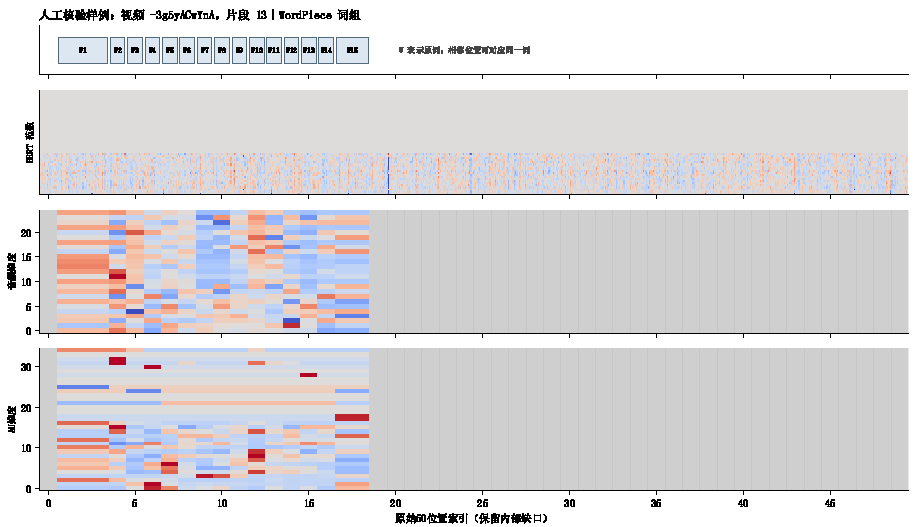
\includegraphics[width=\textwidth]{figures/fig_q1_sample.pdf}
\caption{样本 \texttt{-3g5yACwYnA\$\_\$13} 的位置—时间映射与三路观测。最上一行用 W 编号标出原词，相邻的几个子词可对应同一个词；灰色表示该模态在该位置没有有效观测。声学与动作单元热图按本样本的可观测位置逐维标准化并截断到 $[-3,3]$，只用于展示结构}
\label{fig:q1case}
\end{figure}

图中能看出两个特点。一是三路的有效区间完全对齐，都在前18个正文位置上，之后是整齐的补齐区；二是声学和动作单元热图的第1～3列颜色完全相同，这就是 They've 的三个子词共享同一个词时间窗的直接体现。

\subsection{全量结果与异常核验}\label{sec:q1res}

100条样本的逐条台账见附录\ref{app:A}的表\ref{tab:appA}，包括时长 $D_i$、三个有效长度、词级对齐成功数 $W_i$（拿到时间的词数/原词总数）、处理状态和截断标志。图\ref{fig:q1status}给出了全量的处理状态、对齐分支和有效长度分布。

\begin{figure}[htbp]
\centering
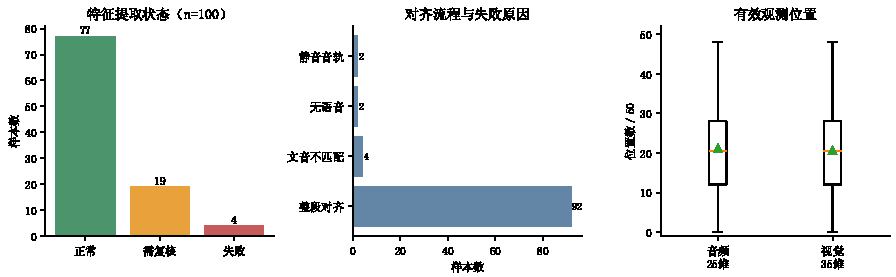
\includegraphics[width=\textwidth]{figures/fig_q1_status.pdf}
\caption{问题一全量结果（100条）：左为处理状态，中为对齐分支与失败原因（“整段对齐”表示走了整段强制对齐流程，不代表每个词都有时间），右为声学、视觉有效位置数的分布}
\label{fig:q1status}
\end{figure}

处理状态为：正常77条、需复核19条、失败4条。异常的几类情况彼此有重叠，不能简单相加，我们把它们分开列在表\ref{tab:q1check}里。

\begin{table}[htbp]
\centering
\caption{问题一的异常与核验（各类之间允许重叠）}
\label{tab:q1check}
\begin{tabularx}{\textwidth}{lr>{\raggedright\arraybackslash}X}
\toprule
检查项 & 数量 & 说明与处理 \\
\midrule
文本截断 & 6段 & 正文子词超过48个，保留截断标志 \\
未全部对齐 & 9段 & 8段完全没有词时间、1段部分词缺失；不补造时间 \\
无达标动作单元帧 & 4段 & OpenFace 阶段找不到满足门槛的帧，记为失败 \\
人工核验 & 31段、583词 & 全部通过；核验结果不改写机器状态 \\
带时间的位置 & 2111个 & 均满足 $0\le s\le e\le D_i$ \\
\bottomrule
\end{tabularx}
\end{table}

9段没有全部对齐的样本里，2段音频里没有语音，2段音轨是静音，4段转写与声音对不上，这8段完全拿不到词时间；另有1段只有8个词中的4个对上，即样本 \texttt{-HwX2H8Z4hY\$\_\$2}。4段失败样本都在这8段之中，而且都卡在 OpenFace 阶段。

这里有一处需要交代的修订。初版导出时，这4段失败样本因为流程在 OpenFace 阶段中断，已经算好的文本矩阵没有保存下来。修订时我们用题目给定的转写和同一版本的 BERT 重新生成了这4段的文本矩阵，而它们的声学、视觉矩阵仍为 None，失败状态也保持不变。另有4段需复核样本保留了文本矩阵，但声学、视觉的可观测位置为0。这4段加上4段失败样本，正好就是那8段完全没有词时间的样本：没有词时间窗，声学和视觉帧也就无处可放。合起来，文本在100段上都有有效位置，声学和视觉各在92段上至少有一个可观测位置。

表\ref{tab:q1check}最后一行只能说明保存的时间没有越出视频边界，并不能说明每个词在语义上都对准了，这也是我们另做人工核验的原因。从全量看，1932个原词中有1820个拿到了时间，占94.2\%。

\subsection{小结}

问题一用强制对齐给定转写的方法求出词级时间，再把声学帧和人脸动作帧按词时间窗池化到BERT子词位置上，得到768、25、35维的三路特征，每个有效位置都能反查到原词、秒数和帧号。100条样本全部保留，失败和异常以显式状态记录；我们宁可让个别位置没有时间，也不为它编一个无法核对的时间。

% ==================================================================
\section{问题二：局部模态缺失下的情感预测}\label{sec:q2}
% ==================================================================

问题二在附件2的50位置特征上，同时预测片段的三分类极性和连续强度，并衡量局部连续缺失对两类输出的影响。本章先说明三种掩码怎么分开，再给出正式模型 PM-B2 和评估面板，然后依次报告基线比较、缺失规律、测试集误差分析和我们做过的改进尝试，最后对附件3推理。

\subsection{数据、标签与三种掩码}\label{sec:q2data}

每条样本在同一条50位置轴上给出文本、声学、视觉矩阵，维度分别为 $50\times768$、$50\times74$、$50\times35$。情感强度 $y_i\in[-3,3]$；类别由原标注固定为负向、中性、正向三类，编码为0、1、2，其中 $y_i=0$ 只属于中性。训练只用训练集的标签，验证集用于选结构、超参数和检查点。

矩阵里的零可能来自补齐填充、原生不可观测或我们施加的遮蔽，因此对样本 $i$、模态 $m$、位置 $t$ 分别记录布局掩码 $\ell_{imt}$、原生可观测掩码 $o_{imt}$ 和人为遮蔽掩码 $s_{imt}$。实际送入模型的是
\begin{equation}\label{eq:mask}
a_{imt}=o_{imt}(1-s_{imt}),\qquad \tilde{\boldsymbol x}_{imt}=a_{imt}\,\frac{\boldsymbol x_{imt}-\boldsymbol\mu_m}{\boldsymbol\sigma_m},
\end{equation}
其中 $\boldsymbol\mu_m$、$\boldsymbol\sigma_m$ 只用训练集中可观测位置估计，标准化以后再把不可观测位置清零。文本掩码排除 \texttt{[CLS]}、\texttt{[SEP]} 和补齐位，声学、视觉掩码由非零行确定。布局掩码 $\ell$ 保留原来的位置范围：序列内部的缺口仍占着原来的序号，不会被挤到序列末尾。三种模态全部不可用时，模型直接返回训练集的类别频率和强度中位数，避免从一个空输入里得出针对具体样本的结论。

\subsection{PM-B2 池化双头模型}\label{sec:pmb2}

模型的思路很朴素：先把每个模态的可观测位置汇总成固定长度的统计量，再用一个小网络同时预测类别和强度。对模态 $m$，在可用位置上求均值和标准差：
\begin{equation}\label{eq:pool2}
\boldsymbol\mu_{im}=\frac{\sum_t a_{imt}\tilde{\boldsymbol x}_{imt}}{\max\!\big(1,\sum_t a_{imt}\big)},\qquad
\boldsymbol d_{im}=\left[\boldsymbol\mu_{im},\ \sqrt{\frac{\sum_t a_{imt}\big(\tilde{\boldsymbol x}_{imt}-\boldsymbol\mu_{im}\big)^{\odot2}}{\max\!\big(1,\sum_t a_{imt}\big)}}\ \right],
\end{equation}
可用位置为空时两项都取零向量。这种池化天然适应缺失：缺了一段，只是参与平均的位置少了，不会像序列模型那样在缺口处读到一串假的零。

三路拼接后的维度为 $2\times(768+74+35)=1754$。PM-B2 用 $1754\to128\to64$ 的两层 ReLU 网络融合，层间 dropout 为0.2；64维共享表示后面接两个独立的线性头，一个输出三类 logits $\boldsymbol z_i$，一个输出强度原值 $u_i$：
\begin{equation}\label{eq:heads}
\begin{gathered}
\boldsymbol p_i=\mathrm{softmax}(\boldsymbol z_i),\qquad \hat c_i=\mathop{\arg\max}_{c\in\{0,1,2\}}p_{ic},\qquad
\hat y_i=3\tanh(u_i),\\
\mathcal{L}=\frac{1}{B}\sum_{i=1}^{B}\Big[-\log p_{i,c_i}+\big|y_i-\hat y_i\big|\Big].
\end{gathered}
\end{equation}
$3\tanh$ 把强度限制在 $[-3,3]$ 内，回归用 L1 损失，与评价指标 MAE 一致。两个输出来自同一个检查点，但分类结果并不由强度的正负号决定，所以会出现“判为中性、强度略偏正”这样的组合，这是两个头各自判断的结果，并非拼接错误。训练设置见表\ref{tab:q2train}。

\begin{table}[htbp]
\centering
\caption{PM-B2 的训练设置}
\label{tab:q2train}
\begin{tabularx}{\textwidth}{l>{\raggedright\arraybackslash}X}
\toprule
项目 & 设置 \\
\midrule
数据 & 附件2 aligned\_50：训练集3395条拟合，验证集728条选型 \\
网络 & 均值+标准差池化 $\to$ 1754 $\to$ 128 $\to$ 64（ReLU，dropout 0.2）$\to$ 分类头 + 强度头 \\
优化 & AdamW，学习率 $3\times10^{-4}$，批大小64，最多30轮 \\
随机种子 & 17、29、43 用于结构比较；专项推理部署 seed 17 \\
检查点选择 & 验证集63档平均 macro-F1 优先，63档平均 MAE 其次，同分取较早轮次 \\
训练遮蔽 & PM-B2 本身不做训练遮蔽；对照模型的缺失增广用固定种子 20260923 生成的双窗口库 \\
复现 & 参数、代码与输入缓存的哈希写入冻结清单 \\
\bottomrule
\end{tabularx}
\end{table}

\subsection{局部缺失面板与评价指标}\label{sec:panel}

正式面板 $\mathcal{K}_{PM}$ 只在被选中的模态里删除一段连续窗口，其余模态保持原样。设某模态原可观测位置的首、尾序号为 $f$、$l$，跨度 $L=l-f+1$。对名义缺失比例 $r\in\{0.1,0.3,0.5\}$，窗口宽度取 $\max(1,\lfloor rL\rfloor)$，起点取头、中、尾三者之一，截出的区间再与 $o_{imt}$ 取交。可观测位置少于两个时不删除，并保证不会把原本可观测的模态整个删空。由于原生缺口、特殊词元和取整的存在，实际删除比例
\begin{equation}\label{eq:rho}
\rho_{im}=\frac{\sum_t o_{imt}s_{imt}}{\max\!\big(1,\sum_t o_{imt}\big)}
\end{equation}
未必等于名义比例，所以后文的10\%、30\%、50\%指的是名义档位。文本的遮蔽不是简单地把缓存的 BERT 向量置零，而是从原始词元输入里移除相应位置，再经同一个冻结的 BERT 重新编码，这样被删掉的词也不会通过上下文“泄漏”到其他位置。验证时统一使用确定的头、中、尾窗口。

被遮蔽模态的非空组合有 $T$、$A$、$V$、$TA$、$TV$、$AV$、$TAV$ 七种，与3种比例、3种位置组合成 $7\times3\times3=63$ 档。每一档都在同一批728条验证样本上计算指标，再对63档等权平均。评价指标为
\begin{equation}\label{eq:metrics}
\begin{gathered}
\mathrm{Acc}=\frac{1}{n}\sum_i\mathbb{1}(\hat c_i=c_i),\qquad
F_{1,\mathrm{macro}}=\frac{1}{3}\sum_{c=0}^{2}\frac{2P_cR_c}{P_c+R_c},\\
\mathrm{MAE}=\frac{1}{n}\sum_i|\hat y_i-y_i|,\qquad
\bar F_{1,63}=\frac{1}{63}\sum_{k=1}^{63}F_{1,k},
\end{gathered}
\end{equation}
其中 $P_c$、$R_c$ 为第 $c$ 类的精确率和召回率，分母为零时该类 F1 记为0；$\overline{\mathrm{MAE}}_{63}$ 同样先逐档再平均。皮尔逊相关系数在预测或真实强度为常数时记为未定义，而不是记为0。

\subsection{基线比较与缺失训练消融}\label{sec:baseline}

表\ref{tab:baselines}列出了在同一正式面板上比较的7个基线：B0 直接输出训练集先验；B1-T、B1-A、B1-V 是单模态池化线性模型；B3 对三个单模态输出做固定权重的决策融合；B1-N 是文本双向 LSTM；B4 是低秩融合\cite{liu2018lmf}。图\ref{fig:baselines}把它们画在同一张图上。

\begin{table}[htbp]
\centering
\caption{正式局部缺失面板上的结构比较（验证集728条、63档；神经网络模型为 seed 17/29/43 的均值 $\pm$ 标准差）}
\label{tab:baselines}
\begin{tabular}{lcc}
\toprule
模型 & 63档平均 macro-F1 & 63档平均 MAE \\
\midrule
B0 训练集先验 & 0.2114 & 0.7690 \\
B1-T 单文本 & 0.4979 & 0.9095 \\
B1-A 单声学 & 0.3526 & 0.8263 \\
B1-V 单视觉 & 0.3455 & 0.7818 \\
B3 决策融合 & 0.4983 & 0.7277 \\
B1-N 文本 BiLSTM & 0.5520 $\pm$ 0.0090 & 0.6523 $\pm$ 0.0144 \\
B4 低秩融合 & 0.5686 $\pm$ 0.0057 & 0.6248 $\pm$ 0.0079 \\
PM-B2 池化双头 & \textbf{0.5752 $\pm$ 0.0013} & \textbf{0.6213 $\pm$ 0.0123} \\
\bottomrule
\end{tabular}
\end{table}

\begin{figure}[htbp]
\centering
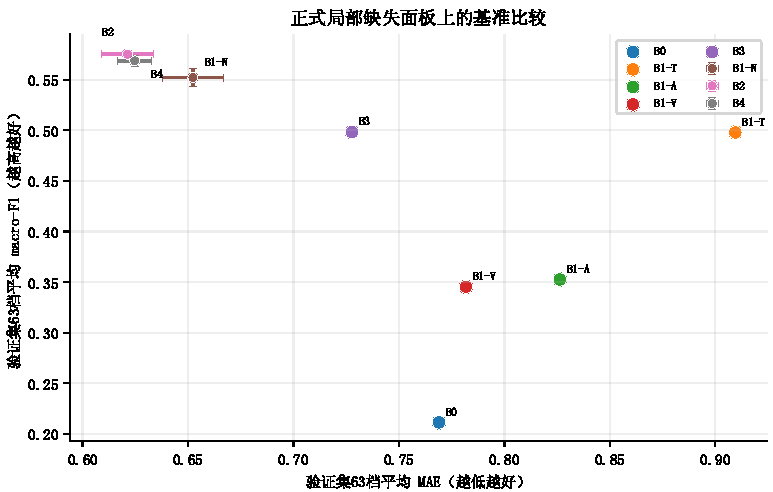
\includegraphics[width=0.8\textwidth]{figures/fig_q2_baselines.pdf}
\caption{各基线在正式面板上的表现（横轴63档平均 MAE，越左越好；纵轴63档平均 macro-F1，越高越好；B1-N、B2、B4 的误差线为三个种子间的标准差，图中 B2 即 PM-B2）}
\label{fig:baselines}
\end{figure}

PM-B2 在 F1 和 MAE 上都是7个模型里最好的，而且三个种子间的 F1 标准差只有0.0013，远小于 B1-N 和 B4。几个单模态基线也很说明问题：只用文本的 B1-T 的 F1 接近0.50，只用声学或视觉的都在0.35左右，只比先验好一截。B0 的 F1 只有0.2114，比三分类随机的1/3还低，因为它永远预测多数类，另外两类的 F1 都是0。

参数更多的时序模型是否值得？我们在同样的学习率和三个种子下做了一个 $2\times2$ 消融：M0 是不做缺失增广、也不显式使用可观测掩码的跨模态时序网络；M1 只加连续遮蔽训练；M2 只让注意力和池化显式使用可观测掩码；M3 两者都用。结果见表\ref{tab:m0m3}。

\begin{table}[htbp]
\centering
\caption{跨模态时序模型的 $2\times2$ 消融（验证集728条、正式面板63档、三种子均值）}
\label{tab:m0m3}
\begin{tabular}{ccccc}
\toprule
配置 & 训练遮蔽 & 显式可观测掩码 & macro-F1 & MAE \\
\midrule
M0 & 否 & 否 & 0.5555 & 0.6295 \\
M1 & 是 & 否 & 0.5630 & 0.6290 \\
M2 & 否 & 是 & 0.5648 & 0.6273 \\
M3 & 是 & 是 & 0.5682 & 0.6195 \\
\bottomrule
\end{tabular}
\end{table}

两个因素各自都有一点帮助，合在一起的 M3 比 M0 的 F1 高0.0127、MAE 低约0.010；按源视频做配对重抽样，F1 差的95\%区间为 $[0.0049,0.0214]$，不跨零。但即便是 M3，F1 也还是比 PM-B2 低0.007；M3 的 MAE（0.6195）比 PM-B2 略低0.0018，这点差距远小于 PM-B2 自身0.0123的种子间波动。在本题的数据量下，更复杂的时序结构没有换来明显的收益，这也是我们最终选 PM-B2 作为正式模型的原因。

\subsection{缺失类型、比例与位置的影响}\label{sec:law}

表\ref{tab:law}按被遮蔽模态、名义比例和位置三个因素，把部署模型（seed 17）在验证集和测试集上的63档结果分组平均；图\ref{fig:law}是对应的图。每个模态组合跨9档平均，每个比例或位置跨21档平均。

\begin{table}[htbp]
\centering
\caption{PM-B2（seed 17）在正式面板上的分组结果}
\label{tab:law}
\begin{tabular}{llcccc}
\toprule
因素 & 档位 & 验证集 F1 & 验证集 MAE & 测试集 F1 & 测试集 MAE \\
\midrule
\multirow{7}{*}{被遮蔽模态} & $T$ & 0.5563 & 0.6487 & 0.5894 & 0.6979 \\
 & $A$ & 0.5975 & 0.6125 & 0.6144 & 0.6500 \\
 & $V$ & 0.5942 & 0.6126 & 0.6156 & 0.6494 \\
 & $TA$ & 0.5583 & 0.6494 & 0.5887 & 0.6985 \\
 & $TV$ & 0.5573 & 0.6488 & 0.5900 & 0.6988 \\
 & $AV$ & 0.5952 & 0.6131 & 0.6162 & 0.6507 \\
 & $TAV$ & 0.5582 & 0.6495 & 0.5908 & 0.6994 \\
\midrule
\multirow{3}{*}{名义比例} & 10\% & 0.5905 & 0.6180 & 0.6141 & 0.6601 \\
 & 30\% & 0.5716 & 0.6300 & 0.6001 & 0.6756 \\
 & 50\% & 0.5595 & 0.6526 & 0.5879 & 0.6978 \\
\midrule
\multirow{3}{*}{位置} & 头 & 0.5761 & 0.6397 & 0.6002 & 0.6778 \\
 & 中 & 0.5734 & 0.6283 & 0.6072 & 0.6678 \\
 & 尾 & 0.5720 & 0.6326 & 0.5948 & 0.6879 \\
\bottomrule
\end{tabular}
\end{table}

\begin{figure}[htbp]
\centering
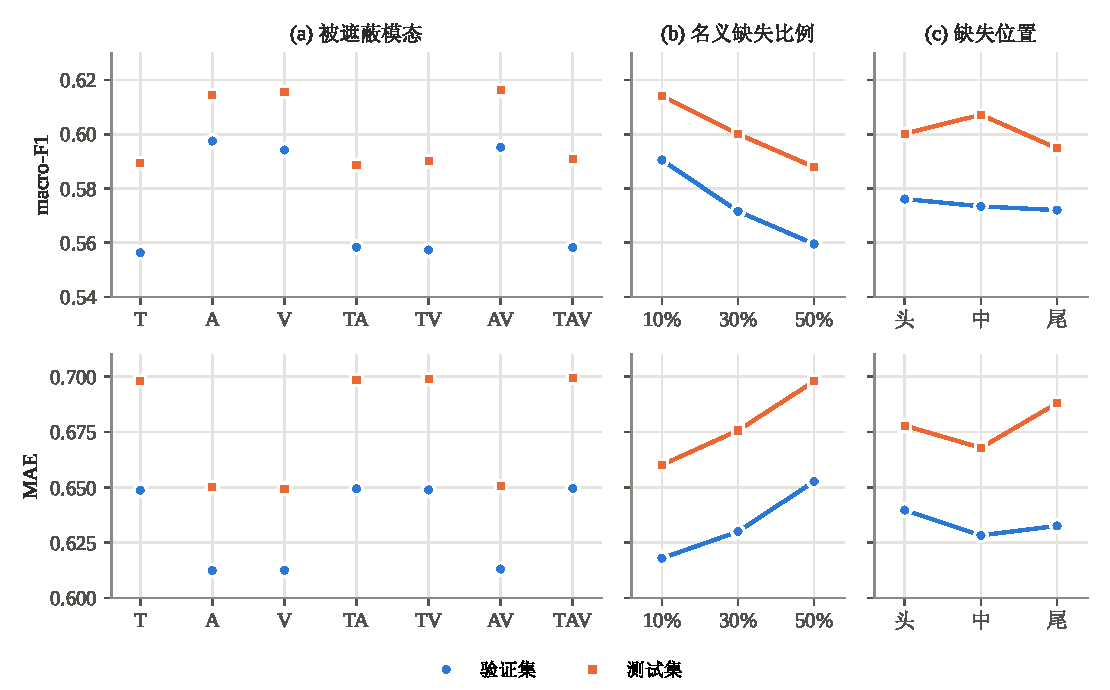
\includegraphics[width=\textwidth]{figures/fig_q2_missing_law.pdf}
\caption{缺失类型、比例与位置对 macro-F1（上）和 MAE（下）的影响（数据同表\ref{tab:law}；模态组合是无序类别，不连线）}
\label{fig:law}
\end{figure}

三个因素的作用大小差别很明显。

\textbf{模态类型影响最大，而且只看“有没有遮文本”。}七种组合清楚地分成两组：凡是遮蔽了文本的（$T$、$TA$、$TV$、$TAV$），验证集 F1 都在0.556～0.558之间；只遮蔽声学或视觉的（$A$、$V$、$AV$），都在0.594～0.598之间，两组相差约0.04，MAE 相差约0.036。组内几乎没有差别，比如在遮蔽文本的基础上再遮蔽声学和视觉（$TAV$），与只遮蔽文本（$T$）相比 F1 几乎不变。这说明当前模型的判断主要依赖文本，声学和视觉局部缺一段对它影响很小。但这不等于声学、视觉在所有样本上都没有用，第\ref{sec:q3}章的逐样本归因会看到少数样本主要依靠它们。

\textbf{缺失比例的影响是单调的。}名义比例从10\%增至50\%，验证集 F1 由0.5905降到0.5595，MAE 由0.6180升到0.6526；测试集的走势完全一致。

\textbf{位置的影响最小，且不稳定。}验证集上头、中、尾的 F1 最大相差0.0041，测试集上相差0.0124，而且两个集合上的排序不一样：验证集是头最好，测试集是中间最好。所以我们不认为存在某个“普遍最要紧”的时间位置。

\subsection{完整输入的结果与错误归因}\label{sec:q2err}

表\ref{tab:q2full}汇总了 PM-B2 在完整输入下的结果。三种子平均、单个部署权重、不同输入条件是三个不同的统计对象，表中分开列出。

\begin{table}[htbp]
\centering
\caption{PM-B2 的完整输入结果}
\label{tab:q2full}
\begin{tabular}{llcccc}
\toprule
对象 & 输入 & Acc & macro-F1 & MAE & Pearson \\
\midrule
验证集三种子均值 & 完整 & 0.6264 & 0.5988$\pm$0.0033 & 0.5998$\pm$0.0128 & -- \\
验证集 seed 17 & 完整 & 0.6277 & 0.6002 & 0.6120 & -- \\
验证集 seed 17 & 63档平均 & -- & 0.5739 & 0.6335 & -- \\
测试集 seed 17 & 完整 & 0.6644 & 0.6147 & 0.6485 & 0.6691 \\
测试集 seed 17 & 63档平均 & -- & 0.6007 & 0.6778 & -- \\
\bottomrule
\end{tabular}
\end{table}

测试集完整输入的混淆矩阵（行为真实的负、中、正，列为预测的负、中、正）及由它算出的各类指标见表\ref{tab:cm}。

\begin{table}[htbp]
\centering
\caption{测试集（727条）完整输入的混淆矩阵与分类指标}
\label{tab:cm}
\begin{tabular}{l|ccc|c|ccc}
\toprule
真实 $\backslash$ 预测 & 负 & 中 & 正 & 合计 & 精确率 & 召回率 & F1 \\
\midrule
负 & \textbf{156} & 23 & 28 & 207 & 0.645 & 0.754 & 0.695 \\
中 & 43 & \textbf{57} & 58 & 158 & 0.442 & 0.361 & 0.397 \\
正 & 43 & 49 & \textbf{270} & 362 & 0.758 & 0.746 & 0.752 \\
\midrule
合计 & 242 & 129 & 356 & 727 & \multicolumn{3}{c}{macro-F1 $=0.6147$} \\
\bottomrule
\end{tabular}
\end{table}

我们按这张表和前面的结果，把错误归纳为以下几类。

\textbf{（1）中性类是主要短板。}负向和正向的召回都在0.75左右，中性只有0.361，F1 只有0.397，拉低了整体的 macro-F1。158条真实中性里，58条被判为正向、43条被判为负向，判对的只有57条。反过来，模型判为中性的129条里也只有57条是对的。换句话说，模型并不是分不清任意两类，而是分不清“中性”和“轻微的正、负”。考虑到中性只对应 $y=0$ 这一个值，而标注是多人评分的平均，“略偏正”和“中性”的边界本身就不清晰，这个问题并不意外。

\textbf{（2）正、负之间也有互相误判。}负向被判为正向的有28条，正向被判为负向的有43条，合计71条，比负、中之间的互相误判（66条）还略多。这部分可能与反讽、转折类句子有关，但仅凭预测与标签的统计，我们不能断定是哪一类语言现象造成的。

\textbf{（3）测试集上强度误差偏大。}测试集完整输入的 MAE（0.6485）高于验证集（0.6120），说明冻结的权重在测试集上的强度误差有所上升，而分类指标反而更好。两者方向不一致，提示强度尺度的校准可能需要单独处理。

\textbf{（4）对文本的依赖过重。}第\ref{sec:law}节的分组结果显示，遮蔽文本是性能下降的主要来源。转写一旦出错，模型很难靠声学和视觉补回来。

\subsection{改进尝试：A–E 五阶段开发实验}\label{sec:ae}

PM-B2 冻结并完成附件3推理以后，我们又只用训练集和验证集、固定 seed 17，做了五个阶段共15种配置的改进尝试，想看看能否在完整输入和缺失两方面同时做得更好。这些实验没有读取测试集和附件3、4。先说结论：完整输入的 F1 确实能提高，但换来的是在更严格的缺失条件下明显退化，没有一个配置在各项指标上全面超过 PM-B2 这条主线，所以正式结果仍以 PM-B2 为准。

\subsubsection{更严格的整模态保留面板}

为了检验这些模型在更极端条件下的表现，我们另设了一个压力面板 $\mathcal{K}_{LH}$：先选一个保留的模态子集 $S\in\{T,A,V,TA,TV,AV,TAV\}$，把 $S$ 以外的模态整路关闭，再只在 $S$ 内施加10\%、30\%、50\%和头、中、尾的连续窗口。它同样是 $7\times3\times3=63$ 档，但含有整路缺失的压力，比正式面板苛刻得多。两个面板的输入分布不同，数值不能互相比较；例如 PM-B2 在正式面板上的0.5752和下面层次头模型在压力面板上的0.4139，并不说明前者“好了0.16”。

\subsubsection{A–C 阶段：文本适配、中性判别与音视频补充}

A 阶段在附件2训练集上用 LoRA\cite{hu2022lora}适配文本表示：在冻结的 BERT 权重 $W_0$ 上学习低秩增量，即 $W=W_0+(\alpha/r)BA$，取秩8、$\alpha=16$、适配器 dropout 0.05。由于要在线更新文本表示，这一阶段直接用原始 text\_bert 的词元编号、注意力掩码和分段输入，而不用原来的 BERT 缓存。我们固定六个组合（冻结或 LoRA、文本单路或三模态、两种学习率），结果见表\ref{tab:stageA}。

\begin{table}[htbp]
\centering
\caption{A 阶段完整输入的验证集结果（728条，seed 17，各取 F1 最优检查点）}
\label{tab:stageA}
\begin{tabular}{lccc}
\toprule
配置 & Accuracy & macro-F1 & MAE \\
\midrule
冻结，文本 & 0.6415 & 0.6036 & 0.5984 \\
冻结，三模态（修复后重训） & 0.6346 & 0.5959 & 0.5953 \\
LoRA，文本，$10^{-4}$ & 0.6538 & 0.6152 & 0.6008 \\
LoRA，三模态，$10^{-4}$（修复后重训） & 0.6442 & 0.6054 & 0.5854 \\
LoRA，文本，$3\times10^{-4}$ & 0.6525 & 0.6052 & 0.5592 \\
LoRA，三模态，$3\times10^{-4}$（修复后重训） & 0.6442 & 0.6203 & 0.5945 \\
\bottomrule
\end{tabular}
\end{table}

LoRA 组整体好于冻结组，F1 最高的是三模态、学习率 $3\times10^{-4}$ 的0.6203。不过这只是单种子的结果，而且冻结组和适配组的训练过程本身也不同，我们不把增益全部归功于 LoRA。表中标注“修复后重训”的三行，是在发现评估代码的问题（见第\ref{sec:fix}节）后重新训练得到的。

B 阶段针对中性类，从 A 阶段的文本 LoRA 模型（学习率 $10^{-4}$）继续训练，试了两条路。B1 按训练集各类样本数 $(967,758,1670)$ 的平方根倒数给分类交叉熵加权。B2 改用层次输出：令 $q=P(\text{中性})$，$r=P(\text{正向}\mid\text{非中性})$，三类概率为
\begin{equation}\label{eq:hier}
(p_{\mathrm{neg}},p_{\mathrm{neu}},p_{\mathrm{pos}})=\big((1-q)(1-r),\ q,\ (1-q)r\big),
\end{equation}
分类损失为中性的二元交叉熵，加上非中性样本的正向二元交叉熵，推理时仍取概率最大的一类。我们把 B2 得到的模型记为 LH-B2，它和 PM-B2 不是同一个模型。两条路都提高了中性召回（由0.337分别升到0.495和0.429），但中性精确率也由0.508降到0.455和0.473，没能同时改善。LH-B2 的完整输入 F1 为0.6244，是各阶段中最高的，因此作为后续 C、D、E 阶段的基础模型。

C 阶段尝试两种音视频补充方式：C1 在 BERT 中间层注入局部音视频残差，C2 在池化特征上分别为分类和回归学习门控。结果见表\ref{tab:stageBC}：C1 的 F1 和 MAE 都不如基础模型；C2 的回归误差下降了，分类却退步。两者都没有形成全面优势，后续没有并入主线。

\begin{table}[htbp]
\centering
\caption{B、C 阶段完整输入的验证集结果（728条，seed 17）}
\label{tab:stageBC}
\begin{tabular}{lcccc}
\toprule
检查点 & Accuracy & macro-F1 & MAE & 中性 F1 \\
\midrule
A 阶段文本模型（B 阶段起点） & 0.6566 & 0.6143 & 0.5877 & 0.4052 \\
B1 加权分类 & 0.6429 & 0.6217 & 0.5692 & 0.4740 \\
B2 层次头（LH-B2） & 0.6484 & \textbf{0.6244} & 0.5987 & 0.4501 \\
C1 局部注入（修复后重训） & 0.6374 & 0.5910 & 0.6225 & 0.3576 \\
C2 两任务独立门控 & 0.6264 & 0.6069 & 0.5857 & 0.4309 \\
\bottomrule
\end{tabular}
\end{table}

\subsubsection{D–E 阶段：表征分解、缺失增广与蒸馏}

D 阶段固定 LH-B2 的文本适配器。D1 只训练小型残差任务头和一个监督对比投影\cite{khosla2020supcon}，正例要求同类且来自不同源视频；D2 借鉴共享/私有表示的思路\cite{hazarika2020misa}，把三模态池化表示拆成共享和私有两支，加上共享对齐、共享与私有的协方差约束和输入重建三个辅助项。E 阶段以 D2 为学生、LH-B2 为固定教师：E0 继续训练但不做缺失增广；E1 在一半样本上按预定的模态组合、比例和窗口合成缺失；E2 在 E1 的基础上再加入对教师分类分布的温度 KL、强度 L1 和批内关系保持项。完整输入与压力面板的结果见表\ref{tab:stageDE}和图\ref{fig:shift}。

\begin{table}[htbp]
\centering
\caption{D、E 阶段在完整输入与整模态保留压力面板上的结果（验证集728条，seed 17；压力面板为63档等权平均）}
\label{tab:stageDE}
\begin{tabular}{lccccc}
\toprule
模型 & 完整 Acc & 完整 F1 & 完整 MAE & 压力 F1 & 压力 MAE \\
\midrule
LH-B2（基础） & 0.6484 & 0.6244 & 0.5987 & 0.4139 & 0.6977 \\
D1 对比头 & 0.6360 & 0.6005 & 0.5912 & 0.4110 & 0.6937 \\
D2 共享/私有 & 0.6401 & 0.6176 & 0.5791 & 0.4286 & 0.7556 \\
E0 无增广 & 0.6113 & 0.5739 & 0.5815 & 0.4500 & 0.7450 \\
E1 缺失增广 & 0.6154 & 0.5578 & 0.5832 & 0.4512 & 0.7279 \\
E2 增广+蒸馏 & 0.6223 & 0.5742 & 0.5891 & 0.4518 & 0.7423 \\
\bottomrule
\end{tabular}
\end{table}

\begin{figure}[htbp]
\centering
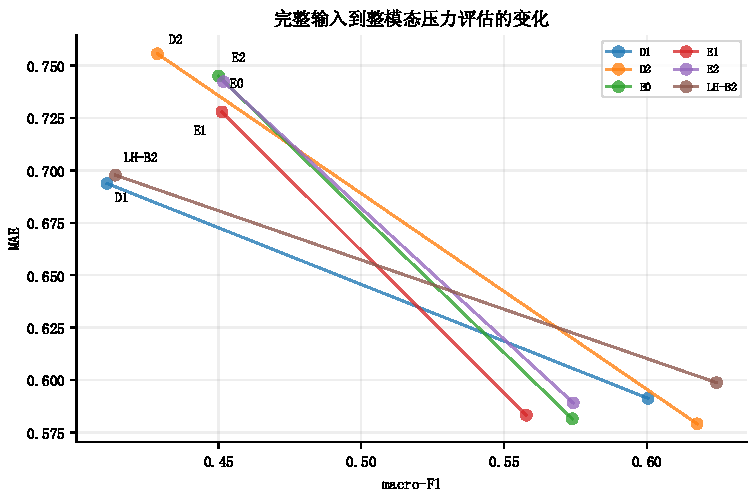
\includegraphics[width=0.78\textwidth]{figures/fig_q2_lh_shift.pdf}
\caption{各检查点从完整输入（右下端点）到压力面板（左上端点）的变化；横轴 macro-F1 越大越好，纵轴 MAE 越小越好}
\label{fig:shift}
\end{figure}

图\ref{fig:shift}里的每条线都从右下往左上走，而且完整输入越好的模型，压力面板上往往越差：LH-B2 的完整输入 F1 最高（0.6244），压力面板 F1 却排在倒数第二（0.4139）；E 阶段三个模型正好相反，压力面板 F1 都在0.45左右（连不做增广的 E0 也是如此），完整输入 F1 却降到了0.56～0.57。再以 D2 为例，它的完整输入 MAE 比 LH-B2 低0.0196，压力面板 F1 高0.0147，可压力面板 MAE 却高了0.0579。

为了判断这些差异是不是抽样波动，我们按验证集的239个源视频做了1000次配对有放回抽样：每次对比较双方用相同的视频组频数，重算各档指标再平均，区间取2.5\%和97.5\%分位数。结果见表\ref{tab:boot}。

\begin{table}[htbp]
\centering
\caption{按源视频配对重抽样的差值（候选减参照；95\%区间，1000次）}
\label{tab:boot}
\begin{tabular}{llcc}
\toprule
比较 & 指标 & 点估计 & 95\%区间 \\
\midrule
\multirow{3}{*}{D2 $-$ LH-B2} & 完整 MAE & $-0.01965$ & $[-0.03470,\,-0.00379]$ \\
 & 压力 F1 & $+0.01469$ & $[+0.00134,\,+0.02738]$ \\
 & 压力 MAE & $+0.05793$ & $[+0.03261,\,+0.08086]$ \\
\midrule
\multirow{2}{*}{E1 $-$ E0} & 压力 F1 & $+0.00118$ & $[-0.01013,\,+0.01259]$ \\
 & 压力 MAE & $-0.01709$ & $[-0.02677,\,-0.00651]$ \\
\midrule
\multirow{2}{*}{E2 $-$ E1} & 压力 F1 & $+0.00056$ & $[-0.00886,\,+0.01117]$ \\
 & 压力 MAE & $+0.01440$ & $[+0.00631,\,+0.02243]$ \\
\bottomrule
\end{tabular}
\end{table}

D2 的三项差异区间都不跨零，说明它确实是用压力面板上的强度误差换来了完整输入的改善。E1 相对 E0 在压力面板上的 MAE 改善是可靠的，F1 的差异则跨零。E2 的蒸馏没有带来可靠的 F1 提升，MAE 反而变差。需要说明，验证集本身参与了检查点选择，这些实验也只有一个训练种子，所以上述区间描述的是已选模型在验证集视频抽样下的波动，不能当作独立测试集上的显著性结论。

\subsubsection{压力面板下的缺失诊断}

我们也在压力面板上看了 E2 的缺失规律。按保留的模态子集分组（表\ref{tab:e2group}），只保留声学或视觉时 F1 只有0.34和0.33左右，保留了文本的各组则在0.518～0.547之间。这再次说明，一旦文本整路不可用，模型就很脆弱。

\begin{table}[htbp]
\centering
\caption{E2 在压力面板上按保留模态分组的结果（每组9档，验证集728条）}
\label{tab:e2group}
\begin{tabular}{lcc@{\hspace{3em}}lcc}
\toprule
保留模态 & F1 & MAE & 保留模态 & F1 & MAE \\
\midrule
$T$ & 0.5179 & 0.7079 & $TA$ & 0.5259 & 0.6664 \\
$A$ & 0.3408 & 0.8805 & $TV$ & 0.5471 & 0.6377 \\
$V$ & 0.3256 & 0.8304 & $AV$ & 0.3623 & 0.8346 \\
$TAV$ & 0.5428 & 0.6388 & & & \\
\bottomrule
\end{tabular}
\end{table}

按名义比例汇总，10\%、30\%、50\%的 F1 依次为0.4623、0.4508、0.4421，MAE 依次为0.7227、0.7383、0.7659；按位置汇总，头、中、尾的 F1 为0.4509、0.4598、0.4446，MAE 为0.7431、0.7362、0.7477。比例的影响单调，位置的影响仍然较小，这与正式面板上的结论一致。这里的“时长”是50个位置上的比例，不能直接换算成秒数。

图\ref{fig:e2scan}把删除率加密扫描到0～1。在0～0.9之间，F1 随删除率缓慢下降、MAE 缓慢上升，删除率超过0.7以后变化明显加快。删除率为1.0时，保留子集里的所有模态都被删空，模型按规则退回训练集先验，F1 与 MAE 回到表\ref{tab:baselines}中 B0 的水平（0.2114和0.7690）。这一点是规则回退的结果，不是局部缺失曲线的自然延伸，图中单独看待。

\begin{figure}[htbp]
\centering
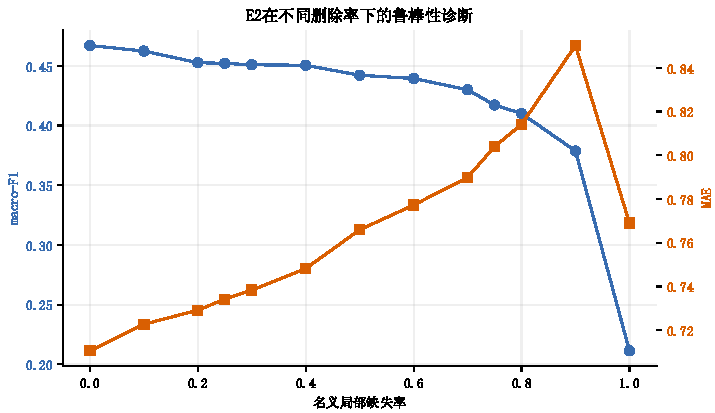
\includegraphics[width=0.78\textwidth]{figures/fig_q2_e2_scan.pdf}
\caption{E2 在不同名义删除率下的 macro-F1（蓝，左轴）与 MAE（橙，右轴），验证集728条，跨保留子集与位置平均}
\label{fig:e2scan}
\end{figure}

\subsubsection{评估代码的两处问题与修正}\label{sec:fix}

开发过程中我们发现评估代码有两处问题：一是不可用模态的数值仍然进入了预测路径；二是压力面板没有真正关闭保留子集以外的模态。受影响的是 A 阶段的三个三模态配置和 C1，它们都已按修正后的输入重新训练，D 阶段的面板也重新评估过；表\ref{tab:stageA}～表\ref{tab:stageDE}中的数值都是修正后的。

修正之后，我们给每次运行加了一道检查：对不可用模态施加任意数值扰动，预测变化必须小于 $10^{-6}$；全空输入必须返回训练集先验；重新加载权重后的预测必须一致。较早的 A、B、D 阶段是事后补做这项检查的，我们不把它们写成当时就已通过。这道检查本身不是新的预测算法，但它决定了上面这些数字能不能信。

\subsubsection{为什么没有替换正式模型}

15种配置里，完整输入 F1 最高的 LH-B2 比 PM-B2（三种子0.5988）高出约0.026，看起来值得替换。我们没有这样做，理由有三：第一，A–E 全部只跑了一个种子，胜出者还没有用 seed 29、43 复核；第二，这些模型在压力面板上普遍退化，说明完整输入的收益可能是以缺失下的稳健性为代价的，而问题二考的恰恰是缺失；第三，测试集已经看过一次，不能再用它来挑选模型。因此附件3的正式预测仍由 PM-B2 给出，A–E 的结果作为改进方向的依据写进论文。

\subsection{附件3推理}\label{sec:att3}

冻结的 PM-B2（seed 17）对附件3的30条样本全部完成了推理，逐条结果见附录\ref{app:B}的表\ref{tab:appB}，分布见图\ref{fig:special}(a)。

\begin{figure}[htbp]
\centering
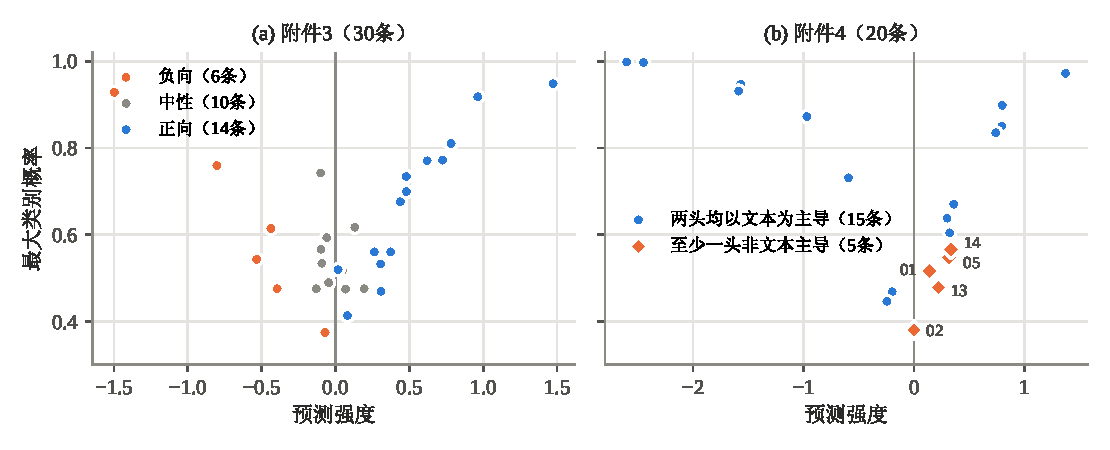
\includegraphics[width=\textwidth]{figures/fig_special_overview.pdf}
\caption{专项测试集的预测概览：(a) 附件3，按预测极性着色；(b) 附件4，按分类与强度两个输出的主导模态区分，橙色菱形为至少一个输出以非文本为主导的样本}
\label{fig:special}
\end{figure}

30条中正向14条、中性10条、负向6条，最大类别概率平均为0.619，其中8条低于0.5。极性与强度的正负号全部一致：判为正向的14条强度都为正（0.018～1.473），判为负向的6条都为负（$-1.497$～$-0.071$），判为中性的10条强度都落在 $[-0.130,0.194]$ 这一窄区间内。三类中中性的平均置信度最低（0.548，正向0.670、负向0.616），这与测试集上中性最难判断的结论是一致的。附件3没有标签，这些统计只能说明模型输出的内部一致性，不代表真实的情感分布或准确率。

\subsection{小结}

问题二的正式模型 PM-B2 结构很简单，却在7个基线和4个时序网络对照中取得了最高的缺失面板 F1，种子间波动也最小。缺失规律上，遮不遮文本是决定性因素，缺失比例的影响单调，位置的影响可以忽略。主要错误集中在中性类。A–E 改进尝试说明，完整输入的提升和缺失下的稳健性之间存在明显的取舍，在单种子证据下我们选择不替换正式模型。

% ==================================================================
\section{问题三：模态归因与可回溯的局部证据}\label{sec:q3}
% ==================================================================

问题三不再训练新模型，而是在问题二冻结的正式模型 PM-B2 上做解释，这样解释的就是实际做预测的那个模型。解释分三层：模态层用 Shapley 值给出三个模态各起了多大作用；位置层用删除检验找出模型最依赖的词或帧，并检验这些证据是否真的影响输出；素材层把证据位置回指到原词、秒数和帧号，由人工核对。

\subsection{解释对象}

问题三使用 PM-B2 为问题三保存的检查点\todo{注明是否与问题二部署的 seed 17 检查点相同}。完整输入下，模型同时输出三类概率 $\boldsymbol p_i$ 和强度 $\hat y_i$。令
\begin{equation}\label{eq:target}
c_i^\star=\mathop{\arg\max}_{c}\ p_i(c)
\end{equation}
为完整输入下的预测类别。后面所有的分类归因都针对这个固定的 $c_i^\star$，删掉某个模态之后即使预测类别变了，我们看的仍是 $c_i^\star$ 这一类的概率。这样做是为了回答一个确定的问题：“模型之所以判为这一类，各部分分别贡献了多少”，而不是每删一次就换一个问题。附件4没有真值，因此本章报告的是预测的结构和解释的一致性，而不是准确率。

\subsection{模态层：八子集精确 Shapley 值}\label{sec:shap}

设模态集合 $N=\{T,A,V\}$。对任一子集 $S\subseteq N$，构造只保留 $S$ 的输入：$S$ 以外模态的数值和可观测掩码同时关闭。分类与强度的“价值函数”定义为
\begin{equation}\label{eq:value}
v_i^{\mathrm{cls}}(S)=p_i\big(c_i^\star\mid S\big),\qquad v_i^{\mathrm{reg}}(S)=\hat y_i(S).
\end{equation}
空集 $\varnothing$ 返回训练集类别先验和强度中位数，与训练、验证、专项推理时的全空处理一致。按固定顺序枚举 $\varnothing,T,A,V,TA,TV,AV,TAV$ 这8个子集，模态 $m$ 的 Shapley 贡献为
\begin{equation}\label{eq:shap}
\phi_{i,m}^h=\sum_{S\subseteq N\setminus\{m\}}\frac{|S|!\,(2-|S|)!}{3!}\Big[v_i^h\big(S\cup\{m\}\big)-v_i^h(S)\Big],\qquad h\in\{\mathrm{cls},\mathrm{reg}\}.
\end{equation}
它的含义是：把三个模态按所有可能的顺序依次加入，模态 $m$ 加入时带来的输出变化的平均值\cite{lundberg2017shap}。三模态只有8个子集，因此可以精确计算，不需要采样近似。计算用64位浮点，并逐样本检查效率恒等式
\begin{equation}\label{eq:eff}
\Big|\sum_{m\in N}\phi_{i,m}^h-\big[v_i^h(N)-v_i^h(\varnothing)\big]\Big|\le10^{-6}.
\end{equation}
728条验证样本和20条附件4样本的两个输出都通过了这项检查。这只说明分摊的算术是对的，并不说明解释符合人对情绪的理解；后者要靠下一节的删除检验和人工核对。

单条样本的贡献可以为负：如果某一路输入反而降低了预测类别的概率，负值本身就是有意义的解释，我们不对它取绝对值后当成支持证据。每个样本的主导模态取贡献最大的模态，分类和强度分别给出；当 $v_i^h(N)-v_i^h(\varnothing)$ 接近零时，各模态的占比没有意义，我们留空而不强行归一化。此外，我们还在预先选定的96条解释样本上换了一种空集基准做敏感性检查，不同基准下的排序变化单独记录。

图\ref{fig:shap}是验证集728条样本上三个模态的平均绝对贡献。

\begin{figure}[htbp]
\centering
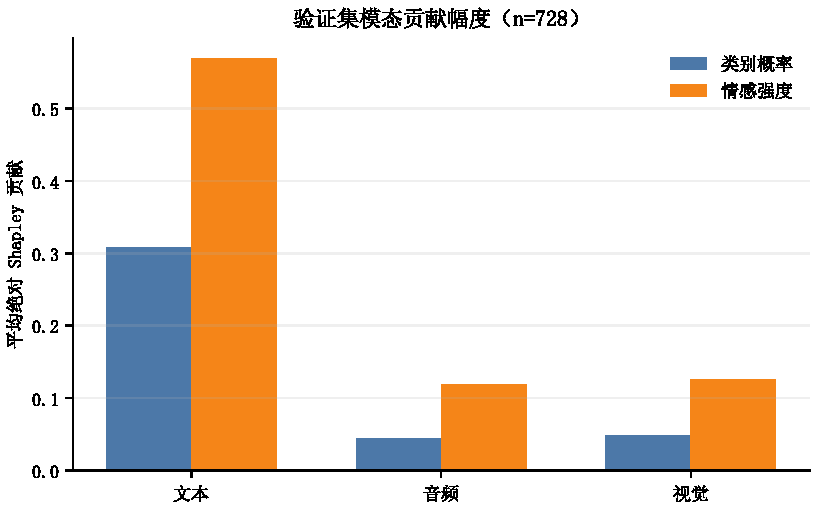
\includegraphics[width=0.66\textwidth]{figures/fig_q3_shapley.pdf}
\caption{验证集728条样本的模态平均绝对 Shapley 贡献（蓝：分类，针对完整输入的预测类别概率；橙：强度输出）}
\label{fig:shap}
\end{figure}

从图中读数，分类输出上文本的平均绝对贡献约为0.31，语音和视觉只有约0.04和0.05，文本是后两者的6～7倍；强度输出上文本约0.57，语音、视觉约0.12和0.13，差距缩小到4～5倍。也就是说，声学和视觉对“有多强烈”的贡献，比对“是正是负”的贡献相对更大。这和直觉一致：语气的轻重、表情的幅度更多反映情感的强弱，而正负方向主要由说了什么决定。这一模态层的结论，也与第\ref{sec:law}节“遮蔽文本是性能下降主因”的结果互相印证。

\subsection{位置层：局部证据与删除检验}\label{sec:local}

先确定解释哪些样本。我们在验证集上按真实类别分层，再对“样本键加固定盐”做 SHA-256 排序，选出96条解释对象。选取过程完全不看模型的预测分数，以免只挑“解释得好看”的样本。

对每个可观测位置，分别删除它的文本、声学或视觉证据，记录目标类概率和强度的变化，作为该位置的局部得分。文本的删除沿用问题二的做法：保留原来的50个位置，把被删的词元换成 PAD 并更新注意力掩码，再经冻结的 BERT 重新编码，而不是把缓存的 BERT 向量置零；声学、视觉则在原位置关闭可观测掩码并重新标准化。令 $R_k$ 为局部得分最高的前 $k$ 个位置，定义
\begin{equation}\label{eq:del}
C_{i,k}^{\mathrm{cls}}=p_i\big(c_i^\star\mid N\big)-p_i\big(c_i^\star\mid N\setminus R_k\big),\qquad
S_{i,k}^{\mathrm{cls}}=p_i\big(c_i^\star\mid N\big)-p_i\big(c_i^\star\mid R_k\big).
\end{equation}
$C$ 衡量删掉这些证据后目标类概率下降多少，越大说明证据越关键；$S$ 衡量只保留这些证据时损失多少，越小说明这几处证据越“够用”\cite{deyoung2020eraser}。强度输出同时保存有符号和绝对值的变化。作为对照，用同样的预算删除得分最低的位置和随机位置；随机位置重复20次，在每个样本内部取平均，这20次是同一样本内的对照，不算20个独立样本。附件4上的结果见图\ref{fig:faith}。

\begin{figure}[htbp]
\centering
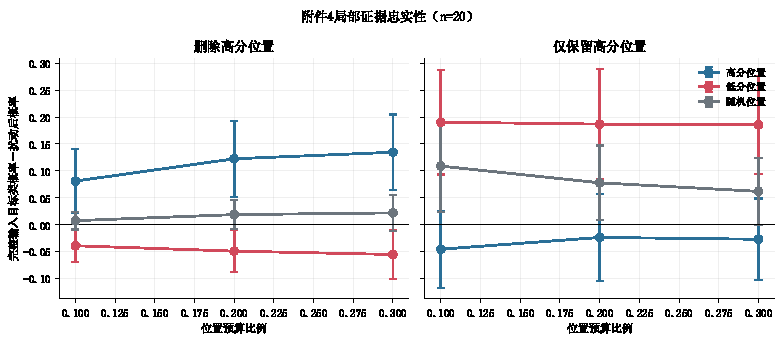
\includegraphics[width=\textwidth]{figures/fig_q3_faithful.pdf}
\caption{附件4（20条）分类证据的删除检验（左）与保留检验（右）。横轴为位置预算占可观测位置的比例；纵轴为完整输入的目标类概率减去扰动后的概率；误差线为20条样本之间的标准差}
\label{fig:faith}
\end{figure}

左图中，三条线分得很开。删除得分最高的位置，目标类概率的下降随预算增加而增大，预算为30\%时平均约0.14；删除随机位置只下降约0.03；删除得分最低的位置，概率反而略有上升（约 $-0.05$），说明这些位置本来是在“拉低”预测类别。右图中，只保留高分位置时概率损失最小（接近0甚至为负），只保留低分位置时损失最大。两张图的方向一致，说明局部得分确实抓住了模型所依赖的位置。不过误差线较宽，20条样本之间的差异不小；而且这些差值说明的是“模型怎么用这些位置”，并不能直接当作这些词在情感上的因果证据。

\subsection{素材层：人工时间核验}\label{sec:review}

局部证据回指到原素材时，用的是问题一建立的“子词位置—词—秒数—帧号”反查链。附件4的人工核验表共有1662个“词—模态”映射行，其中1599行通过、63行被拒绝，被拒绝的63行全部来自样本15：人工核对后确认它的文字与声音对不上，强制对齐给出的时间不可信。另外，样本02从第5个位置起的45行时间整体偏移，按核验结果统一修正了 $-0.55$ 秒。

对样本15，我们保留模型预测和与时间无关的 Shapley 值、删除得分，但从最终展示的时间映射、证据表和解释卡中清除这63行的起止秒数和帧号，只在审计字段里保留工具的原始输出。因此，其余19条可以给出核验过的时间，样本15只给出位置级的解释。模型层面的忠实性检验和素材层面的人工核验是两件事：前者回答“模型是不是这么用的”，后者回答“视频里是不是真有这个”，谁也不能代替谁。

\subsection{附件4的预测与解释}\label{sec:att4}

附件4的20条样本全部输出了三类概率、强度、两个输出的模态贡献和局部证据，逐条汇总见附录\ref{app:C}的表\ref{tab:appC}，分布见图\ref{fig:special}(b)。

20条中正向10条、负向7条、中性3条，平均类别概率为0.717；其中4条（09、10、11、16）强度低于 $-1.5$，是比较强烈的负向，置信度都在0.93以上。分类的主导模态以文本为主（16条），其余为视觉3条（02、05、14）和声学1条（13）；强度的主导模态文本17条、视觉3条（01、05、14）。把两个输出合起来看，有一个很清楚的规律：分类或强度任一输出以非文本为主导的5条样本（01、02、05、13、14），类别概率都不超过0.565，平均只有0.497；两个输出都以文本为主导的15条，平均为0.790。也就是说，当模型主要靠声音或画面做判断时，它自己也没那么有把握。这些样本正是最值得人工回看的。

题目要求给出典型样本的解释卡。以样本01为例，解释卡见表\ref{tab:card}。

\begin{table}[htbp]
\centering
\caption{解释卡示例：附件4样本01}
\label{tab:card}
\begin{tabularx}{\textwidth}{l>{\raggedright\arraybackslash}X}
\toprule
项目 & 内容 \\
\midrule
预测极性与强度 & 中性；强度 $+0.137$（精确值0.1368） \\
三类概率 & 负向0.1154，中性0.5162，正向0.3684 \\
主要参考模态 & 分类：文本；强度：视觉 \\
模态作用程度 & 分类 $\phi^{\mathrm{cls}}_{T},\phi^{\mathrm{cls}}_{A},\phi^{\mathrm{cls}}_{V}=$ \todo{从解释 CSV 抄录}；强度 $\phi^{\mathrm{reg}}_{T},\phi^{\mathrm{reg}}_{A},\phi^{\mathrm{reg}}_{V}=$ \todo{从解释 CSV 抄录} \\
文本关键证据 & Replacing（0.501–0.942 s），timing（2.726–3.007 s）等；对应子词位置 \todo{位置号} \\
声学、视觉证据 & 与上述词时间窗对应的声学帧与视频帧 \todo{视频帧号} \\
时间核验 & 人工核验通过 \\
读法 & 分类主要依据文本，但文本没有把预测推向明确的正负（中性0.52对正向0.37）；强度的主导模态是视觉，给出的是轻微的正值 \\
\bottomrule
\end{tabularx}
\end{table}

这张卡说明了一个有代表性的情况：两个输出头的主导模态不同。分类主要看文本，而“Replacing”“timing”这类词本身没有明显的情感倾向，分类落在中性也就不奇怪；强度则主要由视觉决定，结果是一个轻微的正值。这里的词时间是原素材上的定位，不是这个词单独的情感标签。

题目还要求展示主导模态内局部片段的重要性分布。图\ref{fig:localimp}给出样本01在文本模态上逐位置的局部得分。

\IfFileExists{figures/fig_q3_local_importance.pdf}{%
\begin{figure}[htbp]
\centering
\includegraphics[width=\textwidth]{figures/fig_q3_local_importance.pdf}
\caption{附件4样本01文本模态的逐位置局部得分（横轴为子词位置，标注原词）}
\label{fig:localimp}
\end{figure}}{%
\begin{figure}[htbp]
\centering
\fbox{\parbox{0.9\textwidth}{\centering\vspace{1.2cm}\todo{用解释 CSV 中样本01文本模态的逐位置局部得分画柱状图（横轴子词位置并标注原词），保存为 figures/fig\_q3\_local\_importance.pdf 后重新编译}\vspace{1.2cm}}}
\caption{附件4样本01文本模态的逐位置局部得分}
\label{fig:localimp}
\end{figure}}

\subsection{错误归因}\label{sec:q3err}

\textbf{（1）解释会如实暴露模型对文本的依赖。}绝大多数样本以文本为主导，这是模型真实的行为，解释只是把它说了出来。反过来看，如果某条样本的转写有错，模型大概率会跟着错，而解释卡上会写着“文本主导”，读者据此就知道应该先核对转写。

\textbf{（2）非文本主导的样本置信度偏低。}第\ref{sec:att4}节的5条样本类别概率都不超过0.565，其中样本02只有0.380，基本处在“猜”的状态。对这类样本，解释给出的主导模态本身也不太稳定，更适合作为“请人工复核”的提示，而不是结论。

\textbf{（3）证据时间受强制对齐质量限制。}样本15的文字与声音对不上，时间全部作废；样本02有整体0.55秒的偏移。1662行中有108行（6.5\%）需要拒绝或修正，说明自动对齐的时间不能不经核对就直接当证据用。

\textbf{（4）删除检验的差异在样本间波动较大。}图\ref{fig:faith}的误差线较宽，低预算时高分位置曲线的下沿已接近随机位置，说明样本之间差异不小。20条样本的结论在方向上是清楚的，但幅度还需要更多样本来确认。

\subsection{小结}

问题三在不改动模型的前提下，从模态、位置、素材三层给出了解释。精确 Shapley 值的效率恒等式在全部样本上成立；删除检验显示高分位置确实比随机位置更影响预测；人工核验拒绝了不可信的时间，而没有为它们编造秒数。附件4的20条中，以非文本为主导的样本置信度明显偏低，这为人工复核提供了一个简单实用的筛选依据。

% ==================================================================
\section{模型评价}\label{sec:eval}
% ==================================================================

\subsection{模型的优点}

\begin{enumerate}[label=\arabic*.]
\item \textbf{特征位置都能反查。}问题一用强制对齐给定转写得到词级时间，每个有效位置都挂着“原文字符—词—子词位置—音视频帧”的反查链；典型样本逐词对得上秒数和帧数，31段583个词的人工核验全部通过。
\item \textbf{失败被如实保留。}100条样本一条不删，拿不到时间的位置不补造时间，提取失败的模态记为 None 而不是零，8段没有词时间的样本、4段失败样本都在台账中可查。
\item \textbf{三种零值分开处理。}问题二把补齐填充、原生不可观测、人为遮蔽分成三个掩码，文本遮蔽走重新编码而不是置零，模型和评估都不会把“没有”误读成“为零”。
\item \textbf{简单模型胜在稳定。}PM-B2 在7个基线和4个时序网络对照中缺失面板 F1 最高，三个种子间的标准差只有0.0013；比较时按源视频配对重抽样，没有把重复出现的样本当成独立样本。
\item \textbf{解释分层检验。}问题三的 Shapley 值精确计算且逐样本满足效率恒等式，局部证据有高分、低分、随机三组对照，时间证据再经人工核验，三层检验各管一件事。
\end{enumerate}

\subsection{模型的缺点}

\begin{enumerate}[label=\arabic*.]
\item \textbf{问题一的特征与附件2不通用。}自提的声学特征是25维 eGeMAPS，附件2是74维；两套特征不能互换，问题一的特征质量也就没法用问题二的模型直接检验。
\item \textbf{中性类识别较差。}测试集中性召回只有0.361、F1 只有0.397；B 阶段的加权损失和层次头提高了召回，却降低了精确率，没有同时改善。
\item \textbf{改进实验只有一个种子。}A–E 的15种配置都只跑了 seed 17，胜出者没有复核，蒸馏中关系保持项的单独作用也没有做去除消融。
\item \textbf{专项测试集没有标签。}附件3、4的可信度只能借助附件2上的表现间接判断，附件4的删除检验只有20条样本。
\item \textbf{缺失面板是预设的干预。}63档局部面板和压力面板都是我们设定的缺失方式，真实场景中的缺失未必如此，结论不能直接推广到任意缺失机制。
\end{enumerate}

\subsection{改进方向}

第一，对 A–E 中真正可能改变结论的候选（如 LH-B2、D2）补跑 seed 29 和 43，并对 E2 的关系保持项做单独去除，再用按源视频划分的训练集内交叉验证检验选型是否稳定；在这之前，不用已经看过的测试集或无标签专项集反过来调参。第二，针对中性类，可以把分类阈值和强度预测联合校准，例如让强度接近0且分类置信度低的样本优先判为中性，并在验证集上确定阈值。第三，问题一可以把自提特征接到一个在附件2上训练、但输入维度与之匹配的模型上，才能真正比较不同对齐方式对下游预测的影响。第四，对非文本主导且置信度低的样本，可以设计自动转交人工复核的规则，把问题三的解释直接用到实际流程里。

% ==================================================================
\section*{人工智能工具使用说明}
\addcontentsline{toc}{section}{人工智能工具使用说明}
% ==================================================================

本文的写作过程使用了大语言模型工具：原稿的论文框架、文字初稿及部分图表生成脚本借助 \todo{按实际会话记录填写工具名称与型号，原稿写的是 OpenAI GPT 系列（Codex 会话）}完成；本稿的结构调整、文字改写与 LaTeX 排版借助 Anthropic Claude 完成。文中所有指标、表格和图均来自队伍保存的实验结果文件、冻结清单和人工核验记录，改写过程中没有新增或改动任何实验数值；新增的两张图（图\ref{fig:law}、图\ref{fig:special}）只是把原有表格中的数字重新画成图。参赛队已对照原始记录逐项复核上述内容\todo{复核完成后删去此提示}。若竞赛系统要求提供提示词、模型输出及后续处理方式，另按要求提交。


\bibliographystyle{gmcm}
\bibliography{refs}

\newpage
\appendix
\makeatletter
\renewcommand\secdot{}
\renewcommand\thesubsection{\Alph{section}.\arabic{subsection}}
\makeatother
\addtocontents{toc}{\protect\renewcommand\protect\tocsecdot{}}
% ==================================================================
\section{附件1逐样本特征与对齐台账}\label{app:A}
% ==================================================================

表\ref{tab:appA}逐条给出附件1全部100段视频的处理结果。所有样本的特征维度统一为文本 $50\times768$、声学 $50\times25$、视觉 $50\times35$，对齐粒度为词级（子词位置继承所属原词的时间窗）。表头含义：$D_i$ 为 ffprobe 读取的视频时长；$L_i^T$、$L_i^A$、$L_i^V$ 为按可观测掩码计的有效位置数，“--”表示该模态没有生成矩阵，不等于长度为0的有效特征；$W_i$ 为“拿到时间的词数/原词总数”；状态 O、R、F 分别表示正常、需复核、失败；$C_i=1$ 表示原文正文超过48个子词而被截断。

{\footnotesize\setlength{\tabcolsep}{5pt}\renewcommand{\arraystretch}{1.02}
\begin{longtable}{lrrrrrcc}
\caption{附件1全部100条样本的特征与对齐台账}\label{tab:appA}\\
\toprule
样本键（video\_id\$\_\$clip\_id） & $D_i$/s & $L_i^T$ & $L_i^A$ & $L_i^V$ & $W_i$ & 状态 & $C_i$ \\
\midrule\endfirsthead
\multicolumn{8}{l}{表\ref{tab:appA}（续）}\\\toprule
样本键 & $D_i$/s & $L_i^T$ & $L_i^A$ & $L_i^V$ & $W_i$ & 状态 & $C_i$ \\\midrule\endhead
\bottomrule\multicolumn{8}{r}{续下页}\endfoot
\bottomrule\endlastfoot
\texttt{-3g5yACwYnA\$\_\$13} & 5.514 & 18 & 18 & 18 & 15/15 & O & 0 \\
\texttt{-3g5yACwYnA\$\_\$2} & 9.394 & 17 & 17 & 17 & 14/14 & O & 0 \\
\texttt{-3g5yACwYnA\$\_\$3} & 14.389 & 40 & 40 & 40 & 29/29 & O & 0 \\
\texttt{-3g5yACwYnA\$\_\$9} & 8.817 & 28 & 28 & 28 & 21/21 & O & 0 \\
\texttt{-3nNcZdcdvU\$\_\$5} & 7.868 & 22 & 22 & 22 & 18/18 & O & 0 \\
\texttt{-571d8cVauQ\$\_\$0} & 5.067 & 16 & 16 & 16 & 12/12 & O & 0 \\
\texttt{-571d8cVauQ\$\_\$5} & 15.273 & 48 & 48 & 46 & 43/43 & R & 1 \\
\texttt{-6rXp3zJ3kc\$\_\$8} & 12.805 & 38 & 38 & 37 & 34/34 & R & 0 \\
\texttt{-9y-fZ3swSY\$\_\$0} & 6.833 & 28 & 28 & 28 & 22/22 & O & 0 \\
\texttt{-9y-fZ3swSY\$\_\$4} & 2.821 & 11 & 11 & 11 & 9/9 & O & 0 \\
\texttt{-9y-fZ3swSY\$\_\$8} & 4.989 & 14 & 14 & 13 & 12/12 & R & 0 \\
\texttt{-AUZQgSxyPQ\$\_\$2} & 22.511 & 48 & 48 & 48 & 41/41 & O & 1 \\
\texttt{-HeZS2-Prhc\$\_\$2} & 8.262 & 17 & 17 & 17 & 16/16 & O & 0 \\
\texttt{-HwX2H8Z4hY\$\_\$2} & 3.982 & 12 & 5 & 3 & 4/8 & R & 0 \\
\texttt{-HwX2H8Z4hY\$\_\$5} & 5.653 & 10 & 10 & 3 & 10/10 & R & 0 \\
\texttt{-HwX2H8Z4hY\$\_\$6} & 3.358 & 9 & 9 & 7 & 7/7 & R & 0 \\
\texttt{-HwX2H8Z4hY\$\_\$9} & 7.734 & 24 & 24 & 24 & 22/22 & O & 0 \\
\texttt{-I\_e4mIh0yE\$\_\$1} & 7.622 & 21 & 21 & 21 & 18/18 & O & 0 \\
\texttt{-I\_e4mIh0yE\$\_\$3} & 9.163 & 30 & 30 & 30 & 22/22 & O & 0 \\
\texttt{-MeTTeMJBNc\$\_\$0} & 9.300 & 26 & 26 & 26 & 21/21 & O & 0 \\
\texttt{-MeTTeMJBNc\$\_\$13} & 5.430 & 16 & 16 & 16 & 14/14 & O & 0 \\
\texttt{-MeTTeMJBNc\$\_\$7} & 10.517 & 33 & 33 & 30 & 31/31 & R & 0 \\
\texttt{-NFrJFQijFE\$\_\$1} & 5.746 & 16 & -- & -- & 0/16 & F & 0 \\
\texttt{-NFrJFQijFE\$\_\$2} & 6.856 & 18 & -- & -- & 0/18 & F & 0 \\
\texttt{-RfYyzHpjk4\$\_\$11} & 5.239 & 19 & 19 & 18 & 17/17 & R & 0 \\
\texttt{-RfYyzHpjk4\$\_\$2} & 5.516 & 29 & 29 & 29 & 25/25 & O & 0 \\
\texttt{-RfYyzHpjk4\$\_\$8} & 4.589 & 21 & 21 & 21 & 17/17 & O & 0 \\
\texttt{-THoVjtIkeU\$\_\$12} & 14.896 & 42 & 42 & 42 & 39/39 & O & 0 \\
\texttt{-THoVjtIkeU\$\_\$2} & 4.292 & 11 & 11 & 11 & 10/10 & O & 0 \\
\texttt{-THoVjtIkeU\$\_\$6} & 8.097 & 32 & 32 & 32 & 30/30 & O & 0 \\
\texttt{-UUCSKoHeMA\$\_\$0} & 7.800 & 23 & 23 & 23 & 18/18 & O & 0 \\
\texttt{-UacrmKiTn4\$\_\$10} & 7.362 & 22 & 22 & 22 & 18/18 & O & 0 \\
\texttt{-UacrmKiTn4\$\_\$4} & 4.741 & 15 & 15 & 15 & 14/14 & O & 0 \\
\texttt{-UuX1xuaiiE\$\_\$0} & 3.633 & 12 & 12 & 12 & 9/9 & O & 0 \\
\texttt{-UuX1xuaiiE\$\_\$1} & 10.350 & 33 & 33 & 33 & 27/27 & O & 0 \\
\texttt{-UuX1xuaiiE\$\_\$3} & 4.130 & 9 & 9 & 9 & 9/9 & O & 0 \\
\texttt{-UuX1xuaiiE\$\_\$6} & 8.114 & 23 & 23 & 23 & 22/22 & O & 0 \\
\texttt{-a55Q6RWvTA\$\_\$3} & 22.154 & 48 & 48 & 48 & 65/65 & O & 1 \\
\texttt{-aNfi7CP8vM\$\_\$7} & 8.695 & 23 & 23 & 23 & 18/18 & O & 0 \\
\texttt{-aqamKhZ1Ec\$\_\$0} & 10.967 & 16 & 16 & 16 & 14/14 & O & 0 \\
\texttt{-dxfTGcXJoc\$\_\$0} & 20.500 & 48 & 48 & 35 & 41/41 & R & 1 \\
\texttt{-dxfTGcXJoc\$\_\$1} & 16.161 & 42 & 42 & 42 & 36/36 & O & 0 \\
\texttt{-dxfTGcXJoc\$\_\$2} & 16.698 & 40 & 40 & 40 & 34/34 & O & 0 \\
\texttt{-dxfTGcXJoc\$\_\$6} & 12.735 & 32 & 32 & 32 & 27/27 & O & 0 \\
\texttt{-egA8-b7-3M\$\_\$1} & 10.266 & 22 & 22 & 22 & 20/20 & O & 0 \\
\texttt{-egA8-b7-3M\$\_\$13} & 4.184 & 16 & 16 & 16 & 11/11 & O & 0 \\
\texttt{-egA8-b7-3M\$\_\$16} & 5.538 & 13 & 13 & 13 & 11/11 & O & 0 \\
\texttt{-egA8-b7-3M\$\_\$17} & 7.271 & 19 & 19 & 19 & 16/16 & O & 0 \\
\texttt{-egA8-b7-3M\$\_\$18} & 8.386 & 27 & 27 & 27 & 22/22 & O & 0 \\
\texttt{-egA8-b7-3M\$\_\$20} & 6.645 & 24 & 24 & 24 & 20/20 & O & 0 \\
\texttt{-egA8-b7-3M\$\_\$26} & 6.031 & 19 & 19 & 19 & 15/15 & O & 0 \\
\texttt{-egA8-b7-3M\$\_\$6} & 6.265 & 13 & 13 & 12 & 12/12 & R & 0 \\
\texttt{-egA8-b7-3M\$\_\$9} & 5.090 & 12 & 12 & 12 & 10/10 & O & 0 \\
\texttt{-hnBHBN8p5A\$\_\$6} & 6.401 & 14 & 0 & 0 & 0/13 & R & 0 \\
\texttt{-hnBHBN8p5A\$\_\$7} & 7.372 & 17 & 0 & 0 & 0/13 & R & 0 \\
\texttt{-iRBcNs9oI8\$\_\$3} & 5.621 & 9 & 9 & 9 & 8/8 & O & 0 \\
\texttt{-iRBcNs9oI8\$\_\$6} & 2.903 & 5 & 5 & 5 & 5/5 & O & 0 \\
\texttt{-iRBcNs9oI8\$\_\$7} & 4.104 & 15 & 15 & 15 & 9/9 & O & 0 \\
\texttt{-iRBcNs9oI8\$\_\$8} & 8.093 & 26 & 26 & 26 & 21/21 & O & 0 \\
\texttt{-iRBcNs9oI8\$\_\$9} & 3.416 & 5 & 5 & 5 & 5/5 & O & 0 \\
\texttt{-lzEya4AM\_4\$\_\$5} & 7.675 & 21 & 21 & 21 & 19/19 & O & 0 \\
\texttt{-lzEya4AM\_4\$\_\$6} & 14.792 & 48 & 48 & 48 & 43/43 & O & 0 \\
\texttt{-mJ2ud6oKI8\$\_\$1} & 6.103 & 13 & -- & -- & 0/13 & F & 0 \\
\texttt{-mJ2ud6oKI8\$\_\$2} & 5.731 & 17 & 0 & 0 & 0/11 & R & 0 \\
\texttt{-mJ2ud6oKI8\$\_\$6} & 2.257 & 5 & 5 & 5 & 5/5 & O & 0 \\
\texttt{-mJ2ud6oKI8\$\_\$8} & 4.192 & 11 & 11 & 11 & 11/11 & O & 0 \\
\texttt{-mJ2ud6oKI8\$\_\$9} & 7.033 & 29 & 29 & 29 & 22/22 & O & 0 \\
\texttt{-mqbVkbCndg\$\_\$0} & 6.467 & 17 & 17 & 17 & 12/12 & O & 0 \\
\texttt{-qDkUB0GgYY\$\_\$6} & 4.678 & 18 & 18 & 18 & 16/16 & O & 0 \\
\texttt{-ri04Z7vwnc\$\_\$0} & 2.807 & 8 & -- & -- & 0/8 & F & 0 \\
\texttt{-ri04Z7vwnc\$\_\$2} & 6.027 & 26 & 0 & 0 & 0/16 & R & 0 \\
\texttt{-ri04Z7vwnc\$\_\$5} & 3.545 & 11 & 11 & 11 & 9/9 & O & 0 \\
\texttt{-s9qJ7ATP7w\$\_\$0} & 6.800 & 28 & 28 & 28 & 24/24 & O & 0 \\
\texttt{-s9qJ7ATP7w\$\_\$1} & 4.792 & 12 & 12 & 12 & 11/11 & O & 0 \\
\texttt{-s9qJ7ATP7w\$\_\$4} & 4.427 & 10 & 10 & 10 & 9/9 & O & 0 \\
\texttt{-s9qJ7ATP7w\$\_\$5} & 8.561 & 20 & 20 & 20 & 19/19 & O & 0 \\
\texttt{-s9qJ7ATP7w\$\_\$6} & 2.475 & 5 & 5 & 5 & 5/5 & O & 0 \\
\texttt{-s9qJ7ATP7w\$\_\$7} & 6.966 & 38 & 38 & 28 & 28/28 & R & 0 \\
\texttt{-s9qJ7ATP7w\$\_\$8} & 3.295 & 17 & 17 & 17 & 13/13 & O & 0 \\
\texttt{-t217m2on-s\$\_\$2} & 5.686 & 16 & 16 & 16 & 12/12 & O & 0 \\
\texttt{-t217m2on-s\$\_\$7} & 17.183 & 48 & 48 & 48 & 45/45 & O & 1 \\
\texttt{-tANM6ETl\_M\$\_\$3} & 6.758 & 29 & 29 & 27 & 22/22 & R & 0 \\
\texttt{-tPCytz4rww\$\_\$10} & 4.789 & 15 & 15 & 15 & 12/12 & O & 0 \\
\texttt{-tPCytz4rww\$\_\$11} & 5.467 & 20 & 20 & 20 & 17/17 & O & 0 \\
\texttt{-tPCytz4rww\$\_\$12} & 11.864 & 28 & 28 & 28 & 26/26 & O & 0 \\
\texttt{-tPCytz4rww\$\_\$16} & 7.206 & 17 & 17 & 17 & 16/16 & O & 0 \\
\texttt{-tPCytz4rww\$\_\$18} & 6.645 & 22 & 22 & 22 & 16/16 & O & 0 \\
\texttt{-uywlfIYOS8\$\_\$4} & 6.045 & 22 & 22 & 21 & 18/18 & R & 0 \\
\texttt{-vxjVxOeScU\$\_\$4} & 9.127 & 27 & 27 & 27 & 21/21 & O & 0 \\
\texttt{-wMB\_hJL-3o\$\_\$7} & 6.044 & 23 & 23 & 23 & 22/22 & O & 0 \\
\texttt{-wny0OAz3g8\$\_\$0} & 3.333 & 11 & 11 & 11 & 9/9 & O & 0 \\
\texttt{-wny0OAz3g8\$\_\$1} & 6.844 & 28 & 28 & 27 & 23/23 & R & 0 \\
\texttt{-wny0OAz3g8\$\_\$2} & 6.687 & 28 & 28 & 28 & 23/23 & O & 0 \\
\texttt{-wny0OAz3g8\$\_\$3} & 6.146 & 20 & 20 & 20 & 20/20 & O & 0 \\
\texttt{-wny0OAz3g8\$\_\$5} & 6.912 & 27 & 27 & 27 & 20/20 & O & 0 \\
\texttt{-wny0OAz3g8\$\_\$7} & 8.068 & 31 & 31 & 30 & 29/29 & R & 0 \\
\texttt{-wny0OAz3g8\$\_\$9} & 6.213 & 22 & 22 & 22 & 20/20 & O & 0 \\
\texttt{-yRb-Jum7EQ\$\_\$1} & 29.288 & 48 & 48 & 48 & 49/49 & O & 1 \\
\texttt{-yRb-Jum7EQ\$\_\$5} & 13.169 & 31 & 31 & 31 & 25/25 & O & 0 \\
\texttt{-yRb-Jum7EQ\$\_\$6} & 11.242 & 24 & 24 & 24 & 19/19 & O & 0 \\
\end{longtable}}


% ==================================================================
\section{附件3全量预测}\label{app:B}
% ==================================================================

\begin{table}[H]
\centering
\caption{附件3的30条全量预测（强度为 $[-3,3]$ 尺度，$p_{\max}$ 为三类概率的最大值）}\label{tab:appB}
\begin{tabular}{crrr@{\hspace{2.2em}}crrr}
\toprule
编号 & 极性 & 强度 & $p_{\max}$ & 编号 & 极性 & 强度 & $p_{\max}$ \\
\midrule
01 & 负 & $-0.803$ & 0.759 & 16 & 正 & $1.473$ & 0.948 \\
02 & 中 & $-0.098$ & 0.566 & 17 & 负 & $-0.534$ & 0.543 \\
03 & 中 & $-0.046$ & 0.489 & 18 & 中 & $0.194$ & 0.475 \\
04 & 正 & $0.439$ & 0.676 & 19 & 负 & $-0.395$ & 0.475 \\
05 & 负 & $-1.497$ & 0.928 & 20 & 中 & $-0.092$ & 0.534 \\
06 & 正 & $0.782$ & 0.810 & 21 & 正 & $0.374$ & 0.560 \\
07 & 中 & $0.068$ & 0.474 & 22 & 正 & $0.263$ & 0.560 \\
08 & 正 & $0.018$ & 0.519 & 23 & 中 & $0.131$ & 0.617 \\
09 & 正 & $0.963$ & 0.918 & 24 & 负 & $-0.071$ & 0.374 \\
10 & 中 & $-0.100$ & 0.742 & 25 & 中 & $-0.059$ & 0.593 \\
11 & 中 & $0.047$ & 0.517 & 26 & 正 & $0.480$ & 0.699 \\
12 & 正 & $0.620$ & 0.770 & 27 & 正 & $0.725$ & 0.772 \\
13 & 正 & $0.081$ & 0.413 & 28 & 正 & $0.307$ & 0.532 \\
14 & 负 & $-0.437$ & 0.614 & 29 & 正 & $0.308$ & 0.469 \\
15 & 正 & $0.479$ & 0.734 & 30 & 中 & $-0.130$ & 0.475 \\
\bottomrule
\end{tabular}
\end{table}


% ==================================================================
\section{附件4全量预测与时间核验状态}\label{app:C}
% ==================================================================

附件4没有真值，表中类别概率指预测类别的概率。样本15的文字与声音不符，其词时间被人工核验拒绝，只提供位置级解释。

\begin{table}[H]
\centering
\caption{附件4全部20条的预测与时间核验状态（T、A、V 分别为文本、语音、视觉）}\label{tab:appC}
\begin{tabular}{ccrcccc}
\toprule
样本 & 预测类别 & 强度 & 类别概率 & 分类主导 & 强度主导 & 时间状态 \\
\midrule
01 & 中 & $+0.137$ & 0.516 & T & V & 人工核验 \\
02 & 中 & $-0.001$ & 0.380 & V & T & 人工核验 \\
03 & 负 & $-0.198$ & 0.468 & T & T & 人工核验 \\
04 & 正 & $+0.299$ & 0.638 & T & T & 人工核验 \\
05 & 正 & $+0.315$ & 0.547 & V & V & 人工核验 \\
06 & 正 & $+0.359$ & 0.670 & T & T & 人工核验 \\
07 & 正 & $+0.793$ & 0.850 & T & T & 人工核验 \\
08 & 正 & $+0.323$ & 0.604 & T & T & 人工核验 \\
09 & 负 & $-2.447$ & 0.997 & T & T & 人工核验 \\
10 & 负 & $-1.568$ & 0.947 & T & T & 人工核验 \\
11 & 负 & $-1.586$ & 0.931 & T & T & 人工核验 \\
12 & 负 & $-0.970$ & 0.872 & T & T & 人工核验 \\
13 & 正 & $+0.221$ & 0.478 & A & T & 人工核验 \\
14 & 正 & $+0.335$ & 0.565 & V & V & 人工核验 \\
15 & 正 & $+0.739$ & 0.835 & T & T & 拒绝词时间 \\
16 & 负 & $-2.599$ & 0.998 & T & T & 人工核验 \\
17 & 正 & $+1.371$ & 0.972 & T & T & 人工核验 \\
18 & 中 & $-0.246$ & 0.446 & T & T & 人工核验 \\
19 & 负 & $-0.593$ & 0.731 & T & T & 人工核验 \\
20 & 正 & $+0.798$ & 0.898 & T & T & 人工核验 \\
\bottomrule
\end{tabular}
\end{table}


% ==================================================================
\section{文件、工具版本与运行环境}\label{app:D}
% ==================================================================

\begin{table}[htbp]
\centering
\caption{主要复现文件与工具版本}
\label{tab:appD}
\begin{tabularx}{\textwidth}{l>{\raggedright\arraybackslash}X}
\toprule
类别 & 文件、固定值与用途 \\
\midrule
逐样本特征 & q1\_features.pkl：100条特征、掩码、词级时间映射与提取状态；SHA-256：\texttt{\small 000a842110539f9e ce45e6cedd666a60 d02994728c9e4bd8 0037f261356fe798} \\
核验台账 & q1\_summary.csv、q1\_alignment.csv、q1\_review.csv：逐样本状态、子词—时间映射及人工复核记录 \\
运行清单 & manifest.json、tool\_status.json、python\_versions.json：完成状态、模型与可执行文件哈希、环境版本 \\
文本模型 & bert-base-uncased，revision \texttt{\small 86b5e0934494bd15c9632b12f734a8a67f723594}；冻结，取最后一层隐状态 \\
强制对齐 & WhisperX 3.8.6；对齐模型 jonatasgrosman/wav2vec2-large-xlsr-53-english \\
声学工具 & openSMILE 2.5.1；eGeMAPSv02 低层描述量，25维 \\
视觉工具 & OpenFace 2.2.0；17维动作单元强度 + 18维出现标志 \\
运行环境 & Transformers 4.52.4；PyTorch 2.8.0 \\
问题二、三 & 模型参数、代码与输入缓存的哈希见冻结清单；训练设置见表\ref{tab:q2train} \\
\bottomrule
\end{tabularx}
\end{table}

环境版本用于复现，不同版本的输出不一定完全一致。


\end{document}
